%% March 2018
%%%%%%%%%%%%%%%%%%%%%%%%%%%%%%%%%%%%%%%%%%%%%%%%%%%%%%%%%%%%%%%%%%%%%%%%%%%%
% AGUJournalTemplate.tex: this template file is for articles formatted with LaTeX
%
% This file includes commands and instructions
% given in the order necessary to produce a final output that will
% satisfy AGU requirements, including customized APA reference formatting.
%
% You may copy this file and give it your
% article name, and enter your text.
%
%%%%%%%%%%%%%%%%%%%%%%%%%%%%%%%%%%%%%%%%%%%%%%%%%%%%%%%%%%%%%%%%%%%%%%%%%%%%
% PLEASE DO NOT USE YOUR OWN MACROS
% DO NOT USE \newcommand, \renewcommand, or \def, etc.
%
% FOR FIGURES, DO NOT USE \psfrag or \subfigure.
% DO NOT USE \psfrag or \subfigure commands.
%%%%%%%%%%%%%%%%%%%%%%%%%%%%%%%%%%%%%%%%%%%%%%%%%%%%%%%%%%%%%%%%%%%%%%%%%%%%
%
% Step 1: Set the \documentclass
%
% There are two options for article format:
%
% PLEASE USE THE DRAFT OPTION TO SUBMIT YOUR PAPERS.
% The draft option produces double spaced output.
%

%% To submit your paper:
\documentclass[draft,linenumbers]{agujournal2018}
\usepackage{apacite}
\usepackage{gensymb}
\usepackage{url} %this package should fix any errors with URLs in refs.

%%%%%%%
%\usepackage{trackchanges}
% uncomment the line above to use the TrackChanges package to mark revisions if needed.
% The trackchanges package adds five new LaTeX commands:
%
%  \note[editor]{The note}
%  \annote[editor]{Text to annotate}{The note}
%  \add[editor]{Text to add}
%  \remove[editor]{Text to remove}
%  \change[editor]{Text to remove}{Text to add}
%
% complete documentation is here: http://trackchanges.sourceforge.net/
%%%%%%%

\draftfalse

% Now, type in the journal name: \journalname{<Journal Name>}

% ie, \journalname{Journal of Geophysical Research}
%% Choose from this list of Journals:
%
% JGR-Atmospheres
% JGR-Biogeosciences
% JGR-Earth Surface
% JGR-Oceans
% JGR-Planets
% JGR-Solid Earth
% JGR-Space Physics
% Global Biochemical Cycles
% Geophysical Research Letters
% Paleoceanography
% Radio Science
% Reviews of Geophysics
% Tectonics
% Space Weather
% Water Resource Research
% Geochemistry, Geophysics, Geosystems
% Journal of Advances in Modeling Earth Systems (JAMES)
% Earth's Future
% Earth and Space Science
% Geohealth
%

\journalname{JGR-Oceans}


\begin{document}

%  Title
%
% (A title should be specific, informative, and brief. Use
% abbreviations only if they are defined in the abstract. Titles that
% start with general keywords then specific terms are optimized in
% searches)
%
%% ------------------------------------------------------------------------ %%

% Example: \title{This is a test title}

\title{The Seasonal Cycle of Significant Wave Height in the Ocean:  Local vs Remote Forcing}

%% ------------------------------------------------------------------------ %%
%
%  AUTHORS AND AFFILIATIONS
%
%% ------------------------------------------------------------------------ %%

% Authors are individuals who have significantly contributed to the
% research and preparation of the article. Group authors are allowed, if
% each author in the group is separately identified in an appendix.)

% List authors by first name or initial followed by last name and
% separated by commas. Use \affil{} to number affiliations, and
% \thanks{} for author notes.
% Additional author notes should be indicated with \thanks{} (for
% example, for current addresses).

% Example: \authors{A. B. Author\affil{1}\thanks{Current address, Antartica}, B. C. Author\affil{2,3}, and D. E.
% Author\affil{3,4}\thanks{Also funded by Monsanto.}}

\authors{Luke Colosi\affil{1}, Ana B. Villas B\^oas\affil{1}, Sarah T. Gille\affil{1}}


% \affiliation{1}{Scripps Institution of Oceanography, La Jolla, California}
% \affiliation{2}{Second Affiliation}
% \affiliation{3}{Third Affiliation}
% \affiliation{4}{Fourth Affiliation}

\affiliation{1}{Scripps Institution of Oceanography, La Jolla, California}
%(repeat as many times as is necessary)

%% Corresponding Author:
% Corresponding author mailing address and e-mail address:

% (include name and email addresses of the corresponding author.  More
% than one corresponding author is allowed in this LaTeX file and for
% publication; but only one corresponding author is allowed in our
% editorial system.)

% Example: \correspondingauthor{First and Last Name}{email@address.edu}

\correspondingauthor{Sarah T. Gille}{sgille@ucsd.edu}
\correspondingauthor{Ana B. Villas B\^oas}{avillasb@ucsd.edu }

%% Keypoints, final entry on title page.

%  List up to three key points (at least one is required)
%  Key Points summarize the main points and conclusions of the article
%  Each must be 100 characters or less with no special characters or punctuation

\begin{keypoints}
\item Increases in significant wave height (SWH) during boreal and austral spring and summer months is present in most wind anomaly regions
\item  Magnitude of SWH increase is determined by local conditions within wind anomaly region
\item  Probability of swell decreases during wind anomaly events implying SWH increase occurs due to locally forced waves
\end{keypoints}

%% ------------------------------------------------------------------------ %%
%
%  ABSTRACT
%
%
%% ------------------------------------------------------------------------ %%


\begin{abstract}

Significant wave height (SWH) provides insight about the interactions between the ocean and the atmosphere. In the Northern and Southern Hemispheres, wave heights have been observed to undergo an annual sinusoidal cycle in response to seasonal changes in storm patterns. In the California coast region, local expansion fan wind events lead to deviations in significant wave height during boreal spring and summer. Other coastal regions where supercritical channel flows occur due to coastal topography and atmospheric forcing during the early summer months include eastern boundary regions of ocean basins, the south Caribbean, and West Arabian Sea. Here, intraannual variability of surface gravity waves is analyzed globally in SWH and wind speed data, using over two decades of satellite-derived SWH and wind data. The location at which surface waves are generated is used for validation of mechanisms driving wave characteristics. Phasing of the SWH seasonal cycle reveals that the primary hemisphere dominating the wave field has an abrupt and rough boundary through the equatorial region due in part to topography causing shadowing of waves. In summer wind anomaly (SWA) regions, the fraction of wave variability attributed to local wind events varies depending on local conditions. Global maps of probability of swell based on wave age confirm that wind anomaly regions typically have locally forced waves during the spring and summer months.
% 250 word limit for JGR-Oceans; current length is within this limit.
\end{abstract}


%% ------------------------------------------------------------------------ %%
%
%  TEXT
%
%% ------------------------------------------------------------------------ %%


\section{Introduction}

Surface gravity waves are fundamental to our understanding of the interactions between the ocean and atmosphere, including the exchange of momentum, heat, gasses, and energy between the atmosphere and the ocean \cite{cavaleri2012wind}. Gravity waves are commonly categorized by wave period and generation mechanism \cite{munk1951origin}. In this study, we investigate ordinary surface waves, which are classified as having wave periods between 1 to 30 seconds and being predominantly generated by wind. Over the past half century, satellite remote sensing has provided a global perspective on the large scale temporal and spatial variability of these waves. Present altimeters, radiometers, and scatterometers are capable of repeatedly measuring wind speed and significant wave height (SWH) globally with spatial resolution on the order of 100km along swath or altimeter track.

%With the use of satellite altimeters and radiometers or scatterometers, sea surface height and wind speed respectively have been able to be measured on a global scale and over large time periods with spatial resolutions on the order of 100km along swath or altimeter footprint tracks on the ocean surface. The presence of waves on the ocean surface modifies the shape of the altimeter radar return allowing wave conditions to be estimated. One of these conditions includes the bulk parameter called significant wave height (SWH). SWH is defined as the average crest-to-tough height of the 1/3 highest waves within the wave field \cite{ardhuin2015ocean}. This definition corresponds roughly to the visual impression of wave height \cite{ardhuin2015ocean} over the entire satellite's footprint. 

%Significant wave height (SWH) is an available metric for expressing, sub-optimally, the interaction between the atmosphere and ocean. This interaction in its simplest form consists of near surface wind blowing over an area of ocean for a certain duration leading to a transfer of momentum from the atmosphere into the ocean. This consequently generates ordinary surface gravity waves. Once fully-developed, these waves are classified as remotely forced waves and will propagate throughout ocean basins. 

Sufarce waves are generated by the wind and can propagate long distances across the oceans (Snodgrass et al, 1966. Due to the seasonality of storm systems which generate remotely forced waves, SWH varies seasonally, and is expected to have higher values in winter and lower values in summer months. Thus, the long-term temporal variability of SWH is expected to be marked by a sinusoidal cycle with approximate period of 365 days which is referred to as the seasonal or annual cycle. For example, \citet{echevarria2019seasonal} applied a principal component analysis approach to a global wind wave hindcast developed by the Centre for Australian Weather and Climate Research (CAWCR) and found that most of the variance in SWH was explained by seasonal cycle. 
%The annual cycle is present in the intraannual variability for the large majority of world oceans that has exposure to remotely forced waves propagating from high to mid-latitude storm systems because remotely forced waves primarily dominates wave fields globally. Domination of wave field by remotely forced waves refers to the majority of the energy within the wave field originates from remotely storm systems. 
%The annual cycle accounting for the large percentage of variability present in SWH time series for the majority of the ocean has been investigated by \citet{echevarria2019seasonal} through principal component analysis of global wind wave hindcast developed by the Centre for Australian Weather and Climate Research (CAWCR). They found that the first two empirical orthogonal functions accounted for $>90\%$ of the variation present in the seasonal climatology time series \cite{echevarria2019seasonal} and well reproduce the seasonal cycle. 

%This means that a majority of the energy within the wave field originates from remotely storm systems and is therefore associated with remotely forced waves. These high energy remotely forced wave dominate the wave field. However, at times the energy inputted into the wave from local wind events overwhelms the remotely forced wave energy and high energy locally forced wind waves dominate the wave field. 

However, many regions of the world oceans have wave fields heavily influenced by other physical phenomena which cause SWH variability not explained by the seasonal cycle. Other variability occurs for a wide variety of reasons linked to different atmospheric forcing mechanisms on meso and sub-mesoscales. One common source of variability unexplained by the seasonal cycle is produced by wind-seas or locally forced waves which can result in deviations from the SWH seasonal cycle. \citet{villas2017characterization} analyzed a distinct deviation occuring in the California coast region due to a local wind phenomena call expansion fan winds (EFWs) \cite{winant1988marine}. This deviation is characterized as an increase or simply a bump in SWH during the spring and early summer months due to local EFW events generating locally forced waves that dominate the wave field \cite{villas2017characterization}.   

EFWs form due to atmospheric conditions and coastal topography present in the eastern boundary current region of the California coast. During boreal spring and summer, the northwest Pacific Ocean frequently has a high pressure system sitting just off the coast of northern California and Oregon. This high pressure system is adjacent to a low pressure thermal low over the western US. From the balance between the pressure gradient force pointing from the high to low pressure systems and the Coriolis force in the atmosphere counteracting this force, an anticyclonic geostrophic atmospheric flow is generated which drives southward winds along the coast of California. Due to the coast mountain range in the northern and central parts of California and an inversion layer capping the marine layer, a boundary interface just below the height of the coastal mountain range, a supercritical wind channel forms. This wind channel polarizes the wind direction parallel to the coast. In addition, wind speed increases as the wind passes along the coast through capes which are swooping bays found on the coast of California. As the winds propagate down the coast and approaches a cape, compression (deceleration) regions form upwind of the cape while expansion (acceleration) regions form downwind of the cape generating high wind speeds \citealp{winant1988marine,taylor2008northerly}. This amplification of wind speed and polarized direction generates wind speeds greater than expected in the geostrophic wind field predictions. These strong wind blowing down the California coast influences the wave field significantly. The energy inputted into the wave field from local EFW events overwhelms the remotely forced wave energy resulting in locally forced waves dominating the wave field. Therefore, the local EFW events produce an increase in SWH observed in climatological time series analysis as deviation from the seasonal cycle during the late spring and early months. These locally forced waves have been directly linked to the local EFW event \cite{villas2017characterization}.

%This results in choppy surface ocean conditions near the coast. 

%As the predominant northerly (blows from north to south) winds off the California coast in the spring and summer time travels south (due to a high pressure system off the pacific northwest and a thermal low (low pressure system) in the west US region) , the coastal topography and a low-level inversion capping the marine layer create a boundary interface below the height of the coastal mountain range causes an amplification in wind speed (greater than geostrophic wind field predictions) and wind direction to be parallel to the coastline in what is know as a supercritical channel flow in the atmosphere. 

This same supercritical channel flow has been hypothesized by \citet{winant1988marine} to be present in other oceanic regions that have coastal topography and atmospheric conditions similar to California. These regions include the west coast of Australia, the coast of Namibia in southern Africa, the coast of Chile, the southern Caribbean sea, the northwest coast of Africa near Morocco, and in the Arabian sea near the tip of Somalia. These regions are a combination of eastern boundary current regions (EBRs), monsoon regions, and others. Hereon they will be referred collectively as summer wind anomaly (SWA) regions. 

By analyzing intraannual variability of SWH for surface gravity waves and wind speed (WSP) on a global scale from 1993 to 2015 using satellite remote sensing, we investigate SWA regions to determine if the same seasonal cycle deviation as in the California Coastal region is present and if a corresponding maximum in wind speed seasonal cycle is correlated to the SWH deviation. In addition, the structural distribution of the parameters of the seasonal and semi-seasonal cycle on a global scale is explored in order to give insight into the general forcing mechanisms and parameters of the wave field influencing these deviations in SWH\@. In order to justify that SWH during the spring months in these SWA regions are locally forced, wave age can be used for separating growing seas from fully developed seas for collocated WSP and SWH data. We assessing SWA regions in order to understand remote versus local forcing effects on the dominate characteristics of the wave field in order to understand the wave climate in partially wind-sea dominated regions for practical application for coastal infrastructure and shipping within SWA regions.

This paper is organized as follows. Section 2 explains the data sets used to conduct the time series analysis of global SWH data and the limitations of our analysis. Section 3 explores the general parameters of the annual and semi-annual SWH and WSP models for the entire time series globally as well as regional climatologies in order to demonstrate the correlation between the deviations from the seasonal cycle and the maximum in the WSP seasonal cycle. Section 4 uses wave age in order to illustrate that SWH measurements during the spring and summer months within SWA regions are observing wave fields dominated by locally forced wave rather than remotely forced wave justifying the claim that local wind events are causing the deviation from the seasonal cycle. Section 5 summarizes conclusions.

\section{Methods}

\subsection{Remotely sensed Data}

This study makes use of separate multi-satellite remote sensing products for waves and wind.   

Wave data used in this study are drawn from two decades of cross-calibrated satellite altimeter SWH measurements produced by the Institut fran\c{c}ais de recherche pour l'exploitation de la mer (Ifremer).  Ifremer's along track cross calibrated SWH altimeter data was collected from multiple near pole non-sun synchronous satellites over the time period of 1 January 1993 to 31 December 2015. The along track data were binned onto a 1$^{\circ}$ by 1$^{\circ}$ spatial grid with 1-day temporal resolution. Satellites contributing to the analysis include ERS-1\&2, TOPEX-Poseidon, GEOSAT Follow-ON (GFO), Jason-1, Jason-2, ENVISAT, Cryosat and SARAL AltiKa \cite{Queffeulou2017Global}. To enhance the quality of SWH observations, data screening based on multiple flags and uncertainty of measurements to determine the reliability and viability of each data point was performed. Ifremer SWH data are corrected to agree with in situ buoy observations.

Wind data for this study is from the cross calibrated multi-platform version 2 wind vector analysis data (CCMP2) produced by Remote Sensing Systems. CCMP2's data product is released on a 0.25$^{\circ}$ by 0.25$^{\circ}$ spatial grid with 6 hourly temporal resolution. For this analysis, we averaged CCMP2 winds to a 1$^{\circ}$ by 1$^{\circ}$ spatial resolution and 1 day temporal resolution in order to match the Ifremer data set. The CCMP2 product incorporates measurements from active scatterometers, passive radiometers, in situ buoys, and modelled wind velocity data \cite{Atlas2011Remote}. CCMP reports wind in zonal and meridional components \cite{Atlas2011Remote}, which are used to compute WSP. 

For the climatological analysis, monthly data of SWH and WSP were obtained by averaging over each month throughout the time period.  

The Ifremer SWH product is not co-located temporally with the CCMP2 wind product; typical time differences are on the order of 6 hours. For point-to-point analysis, this would present a major obstacle due to the fact that the sea state including wave height or SWH and atmospheric conditions including WSP are highly variable on time scales of minutes to hours, meaning that SWH and WSP can change significantly within a 6 hour period. Therefore, the WSP measurement at a given location could have no correlation at all to a SWH measurement taken 6 hours later at the same location. The analysis done in this study focuses on monthly averaged SWH and WSP.

%Is it okay that I am leave the discussion about WW3 CFSR data until the discussion section? Or should I bring it up in this section?

\subsection{Annual and Semi-Annual Model and Regional Climatology Analysis}

In order to analyze the annual and semi-annual variability of SWH and WSP, at each grid point, we least-squares fitted SWH and WSP with annual and semi-annual sinusoidal cycles: 
 \begin{equation}
     \mbox{\rm f(t)} = x_0 + x_1\times\sin\left(\frac{2{\pi}t}{T}\right) +  x_2\times\cos\left(\frac{2{\pi}t}{T}\right) + x_3\times\sin\left(\frac{4{\pi}t}{T}\right) + x_4\times\cos\left(\frac{4{\pi}t}{T}\right).
 \end{equation}
Here, T is the duration of the annual cycle (12 months), t is time, and $x_n$ are coefficients for the SWH or WSP model. A linear trend within the SWH and wind speed time series was accounted for within our analysis by detrending the WSP and SWH monthly data before computing the model and its parameters. To inspect the magnitude of the linear trend in the data, the least square fit above with a sixth term accounting for a linear trend was fitted to the data. The coefficient for linear trend term were used to give a rudimentary magnitude and significance of the linear trend. \citet{young2011global} preformed a similar analysis on SWH and WSP data from multiple satellite altimeter missions calibrated and validated by \citet{zieger2009joint}. By using a least square fit accounting for the mean, annual cycle and higher frequency oscillations, the magnitude of the linear trend may be approximated via the slope of the trend. However, this approximations may contain spurious results when noise is present \cite{young2011global}. Fig~\ref{Ifremer_ccmp2_lsf_linear_trend} displays globally the magnitude of the linear trend and illustrates that the magnitude is significantly smaller than than amplitudes of the annual and semi-annual signal as well as the variance of the data. The linear trend magnitudes are slightly less than reported by \citet{young2011global}. Whether the linear trend is an unreal artifact of the cross calibrated multi-platform data sets or is physically authentic, we do not know. However, the linear trend is still removed for completeness. 

\begin{figure}[tbh]
\centering
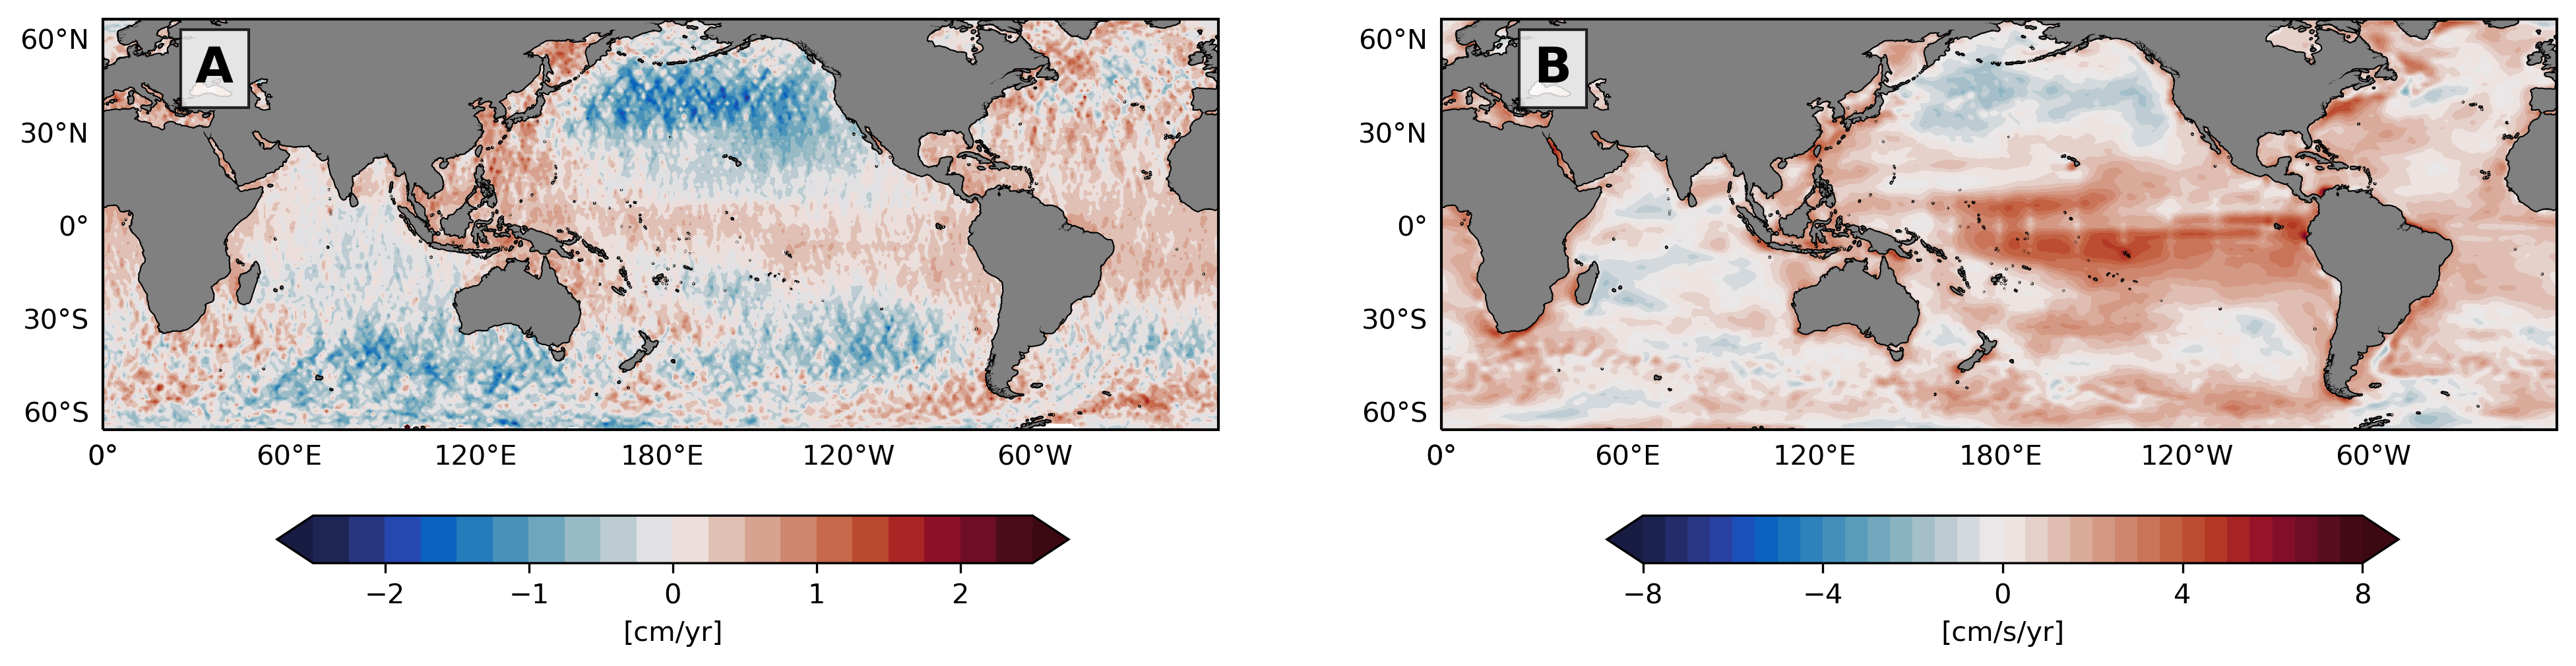
\includegraphics[width=1.0\textwidth]{figs/lsf_parameters/ccmp2_ifremer_linear_trend_magnitude.png}
\caption{Magnitude of linear trend for monthly averaged (A) Ifremer SWH and (B) CCMP2 WSP.}
\label{Ifremer_ccmp2_lsf_linear_trend}
\end{figure}

In order to evaluate the goodness of fit of the model, the root mean square of the residual and coefficient of determination was used. The residual is defined as the difference between the model and the observed data. This method is a rudimentary method of quantifying how well the model fits the observed data and is biased to have high residue in regions with high temporal variability.
\begin{equation}
    \mbox{\rm residual} = \mbox{\rm f(t)} - \mbox{\rm data} 
\end{equation}
\begin{equation}
    \mbox{\rm Root Mean Square Error} = \sqrt{\langle \mbox{\rm residual}^2\rangle} 
\end{equation}
The coefficient of determination is the percent of variance of the data explained by the model and is calculated by taking the ratio of the summed squared error between each data point and the corresponding modelled data divided by the difference between the each data point and the mean value of the data.
\begin{equation}
 r^{2} = 1 - \frac{\rm \sum_{i=0}^{N} residue}{\rm \sum_{i=0}^{N} total} = 1- \frac{\sum_{i=0}^{N} (y_i - f_i)^2}{\sum_{i=0}^{N} (y_i - \overline{y})^2}
 \end{equation}
Here $N$ is equivalent to the the number of observations. The coefficient of determination provides a more robust quantification of the goodness of fit of the model. 

The parameters used to evaluate and compare the seasonal cycles spatially were the amplitude and phase constant. For the amplitude and phase constant of the annual and semi-annual cycle, these parameters were determined by the following equations:
 \begin{eqnarray}
     annual\;amplitude & = & \sqrt{x_1^{2} + x_2^{2}}\\
    semi-annual\;amplitude & = & \sqrt{x_3^{2} + x_4^{2}}\\
     annual\;phase & = & \arctan{\left(\frac{x_2}{x_1}\right)} \\
    semi-annual\;phase & = & \arctan{\left(\frac{x_4}{x_3}\right)}\\
 \end{eqnarray}
For the climatological analysis within SWA regions, SWH and WSP grid points within 4$^{\circ}$ by 4$^{\circ}$ square regions were first temporally averaged into single monthly averages and then spatially averaged. Therefore, we obtain SWH and WSP climatologies for the entire region in order to compare the SWH climatology with the WSP climatology to check for correlation between the SWH deviation and the WSP maximum. The 4$^{\circ}$ by 4$^{\circ}$ regions were picked by looking at seasonally averaged WSP maps within SWA regions. 4$^{\circ}$ by 4$^{\circ}$ regions that had anomalously high WSP and small spatial WSP gradients where chosen as seen in Fig~\ref{reg_clima_nh} and Fig~\ref{reg_clima_sh}. For the northern hemisphere, the seasonal average from the boreal summer was used in order for the high WSP anomaly to be present in SWA regions. Likewise for the southern hemisphere, the seasonal average from the austral summer was used. Small spatial WSP gradient regions were favorable because the climatology analysis should be performed in regions with consistently high amplitude WSP maximum observations in order to have the highest likelihood of the wave field has significant influence by local winds. By spatially averaging over a regions including grid points with high and low amplitude maxima, our averaging would include two domains with very different time variability which would lead to having piece-wise rough climatologies. In addition, decently sized regions to spatially average data were used to bring down some of the noise present in SWA regions.  

%Through the combination of these parameters, many inferences about the underlying dynamics influencing the climatology of specific regions were able to be made. 

Seasonal progression maps of the first two statistical moments for Ifremer SWH and CCMP2 WSP data are computed in order to gain insight into the seasonal evolution and variability of the data (Fig~\ref{Ifremer_swh_seasonal_pro} and Fig~\ref{ccmp2_wsp_seasonal_pro}).

\subsection{Limitations of Data}

The data used in this study have limitations associated with retrieval methods and with multi-satellite intercalibration in order to obtain a continuous or ``gap free" temporal or spatial data set for SWH and WSP. 

Wave on the ocean surface modify the shape of the waveform's returned power due to the varying amount of illuminated area of the sea surface \cite{chelton2001satellite}. Therefore, SWH is estimated by satellite altimeters through measuring the slope of the time evolving returned power from the leading edge of the waveform \cite{chelton2001satellite}. As radiation reflects off backscatterers at the ocean surface with the water, the distance in which the radiation must traverse between the satellite and the sea surface varies due to surface gravity waves. Once the return power begins to return to the satellite, stretching of the leading edge of the return waveform occurs such that early returns come from wave crests while later returns come from wave toughs. This stretching increases as wave height increase leading to a decrease in the slope of the returned power as a function of time. In order to obtain accurate satellite altimetry data of SWH, corrections must be made for accurate determination of the shape of the radar's returned power which include instrument, atmospheric refraction, and sea-state bias corrections as well as external geophysical adjustments \cite{chelton2001satellite}. All these sources of error introduce a certain degree of uncertainty and unreliability with measurements collected by the satellite. However, the satellite altimetry corrections of primary concern for this study are the sea-state biases. The total sea state bias includes the electromagnetic (EM) and skewness biases \cite{chelton2001satellite}. These two errors weaken the reliability of the satellite altimetry observations in regions with high amplitude waves (high wave height) and steep waves which tend to have high frequency. Errors relating to wave steepness are of higher magnitude in SWA regions because locally forced waves tend to be high frequency and consequentially steeper. Errors relating to high wave amplitude occur in SWA in the Southern Hemisphere where the wave field is dominated by large SWH remotely forced waves due to there close proximity to the Southern Ocean. In addition, small-scale surface roughness near the wave crests such as white capping due to local winds amplifies the sea state biases. High surface roughness is common in locally forced wave dominated wave fields. Corrections of sea state bias for SWH have be applied to the satellite altimetry data, however, errors that vary in magnitude geographically are still present in SWH calculations.

In addition, satellite altimetry data in near coastal region on the scales of 10km to 100km should be neglected from the analysis due to the spatial extent of the swath of the satellite and inaccuracies in tidal corrections. The footprint of satellite altimeter is on the order of 10km and averaging occurs over along track distances of 100km in order to increase the precision and accuracy of observations \cite{chelton2001satellite}. This means that the data can be slightly contaminated by the land in regions less than 10km off shore. For tide corrections, the tidal signal, with a surface expression of increased sea surface height in coastal regions, exponentially increase in amplitude when approaching the coast. This tidal signal must be removed from the satellite altimetry measurements in order to remove undesired biases. However, tidal corrections performances still needs improvement. Therefore, coastal region on the length scales quantified by the Rossby radius of deformation away from the coast are neglected. Fortunately, the local wind anomalies persist for several hundreds of kilometer off shore allowing reliable SWH and WSP data satellite data to be recorded \cite{winant1988marine}. 

As discussed, IFREMER SWH data set are cross calibrated between multiple satellite missions. However, in order to compile SWH over several satellite missions for climatological analysis, the data must be validated and verified that the data is homogeneous \cite{queffeulou2004long}. Unvalidated SWH data may contain errors introduced by electronics drift and sensor damage to satellite altimeter which leads to decreased quality of data from discrepancies between satellite missions \cite{queffeulou2004long}. IFREMER SWH data product has been validated by \citet{queffeulou2004long} by comparing SWH measurements with in situ buoy observations for each satellite mission as well as ensured near homogeneity of SWH measurements between satellite missions. For WSP, CCMP2 cross calibration and assimulated surface wind data from satellite remote sensing scatterometers and microwave radiometers from multiple satellite missions use the variation analysis method (VAM) and European Centre for Medium-Range Weather Forecasts (ECMWF) modelled surface winds to validate this product and calibrate it with in situ buoy observations \cite{atlas2011cross}. Therefore, this assimilated and validated gridded product results in high spatial and temporal accuracy suitable for climate studies \cite{Atlas2011Remote}. However, the CCMP2 WSP data set has a few caveats including having spurious trend due to assimilation process of modelled ECMWF data and underestimation of wind speeds in high wind regions due to modelled ECMWF winds tendency to underestimate wind speed \cite{Atlas2011Remote}. Fortunately, the annual and semi-annual cycles are stronger signals present in the WSP climate in SWA regions and would therefore not be considered a spurious trend. However, underestimation of WSP could have effects on the analysis of SWA regions when the wind anomaly occurs. 

Therefore, this study takes advantage of moderate to high spatial and temporal resolution global measurements of SWH and WSP measurements from Ifremer and CCMP2's cross-calibrated multi-satellite mission products to look at the intraannual variability of the SWH seasonal cycle over a 20 year time period; however, with caution due to the known limitations of the data set coming from biases present in both SWH and WSP products especially in SWA regions.

%the stated sea state biases present especially in wind-sea regions for SWH and underestimations of wind field for WSP. 

In addition, this study only focuses on time series analysis of integral or averaged parameter SWH. Other integral parameters that cannot currently be obtained from satellites include peak frequency (or period) and mean wave direction. At any given point on earth, these describe only the dominant wave height, frequency, period, and direction of waves within the wave spectrum that is associated with the highest spectral energy or elevation variance \cite{ardhuin2015ocean}. Therefore, weaker but still prevalent signals from swell and wind-sea waves are suppressed in the result as a result of this analysis. \citet{echevarria2019seasonal} highlight this shortcoming of integral parameters in wave climatology analysis and present a climatological analysis of multimodal directional wave spectrum via principal component analysis of the spectral data from Wave Watch 3 ECMWF reanalysis data. \citet{semedo2011global} also used as well Wave Watch 3 ECMWF reanalysis data in order to analyze the global wave climate. Integral parameters are used in this analysis with the understanding of its limited ability to full describe all modes present in the wave spectrum. This study's results only reflect the analysis of dominant highest spectral energy signal present.

\section{SWH and WSP Intraannual Variability Analysis}

\subsection{Global parameters of Annual and Semi-annual Model and Implications to SWA Regions}

Figure~\ref{Ifremer_ccmp2_lsf_chars} compares the Ifremer SWH annual and semi-annual cycle amplitude and phase with CCMP2 WSP results. Notice that the phase have been converted from radians to months 

\begin{figure}[tbh]
\centering
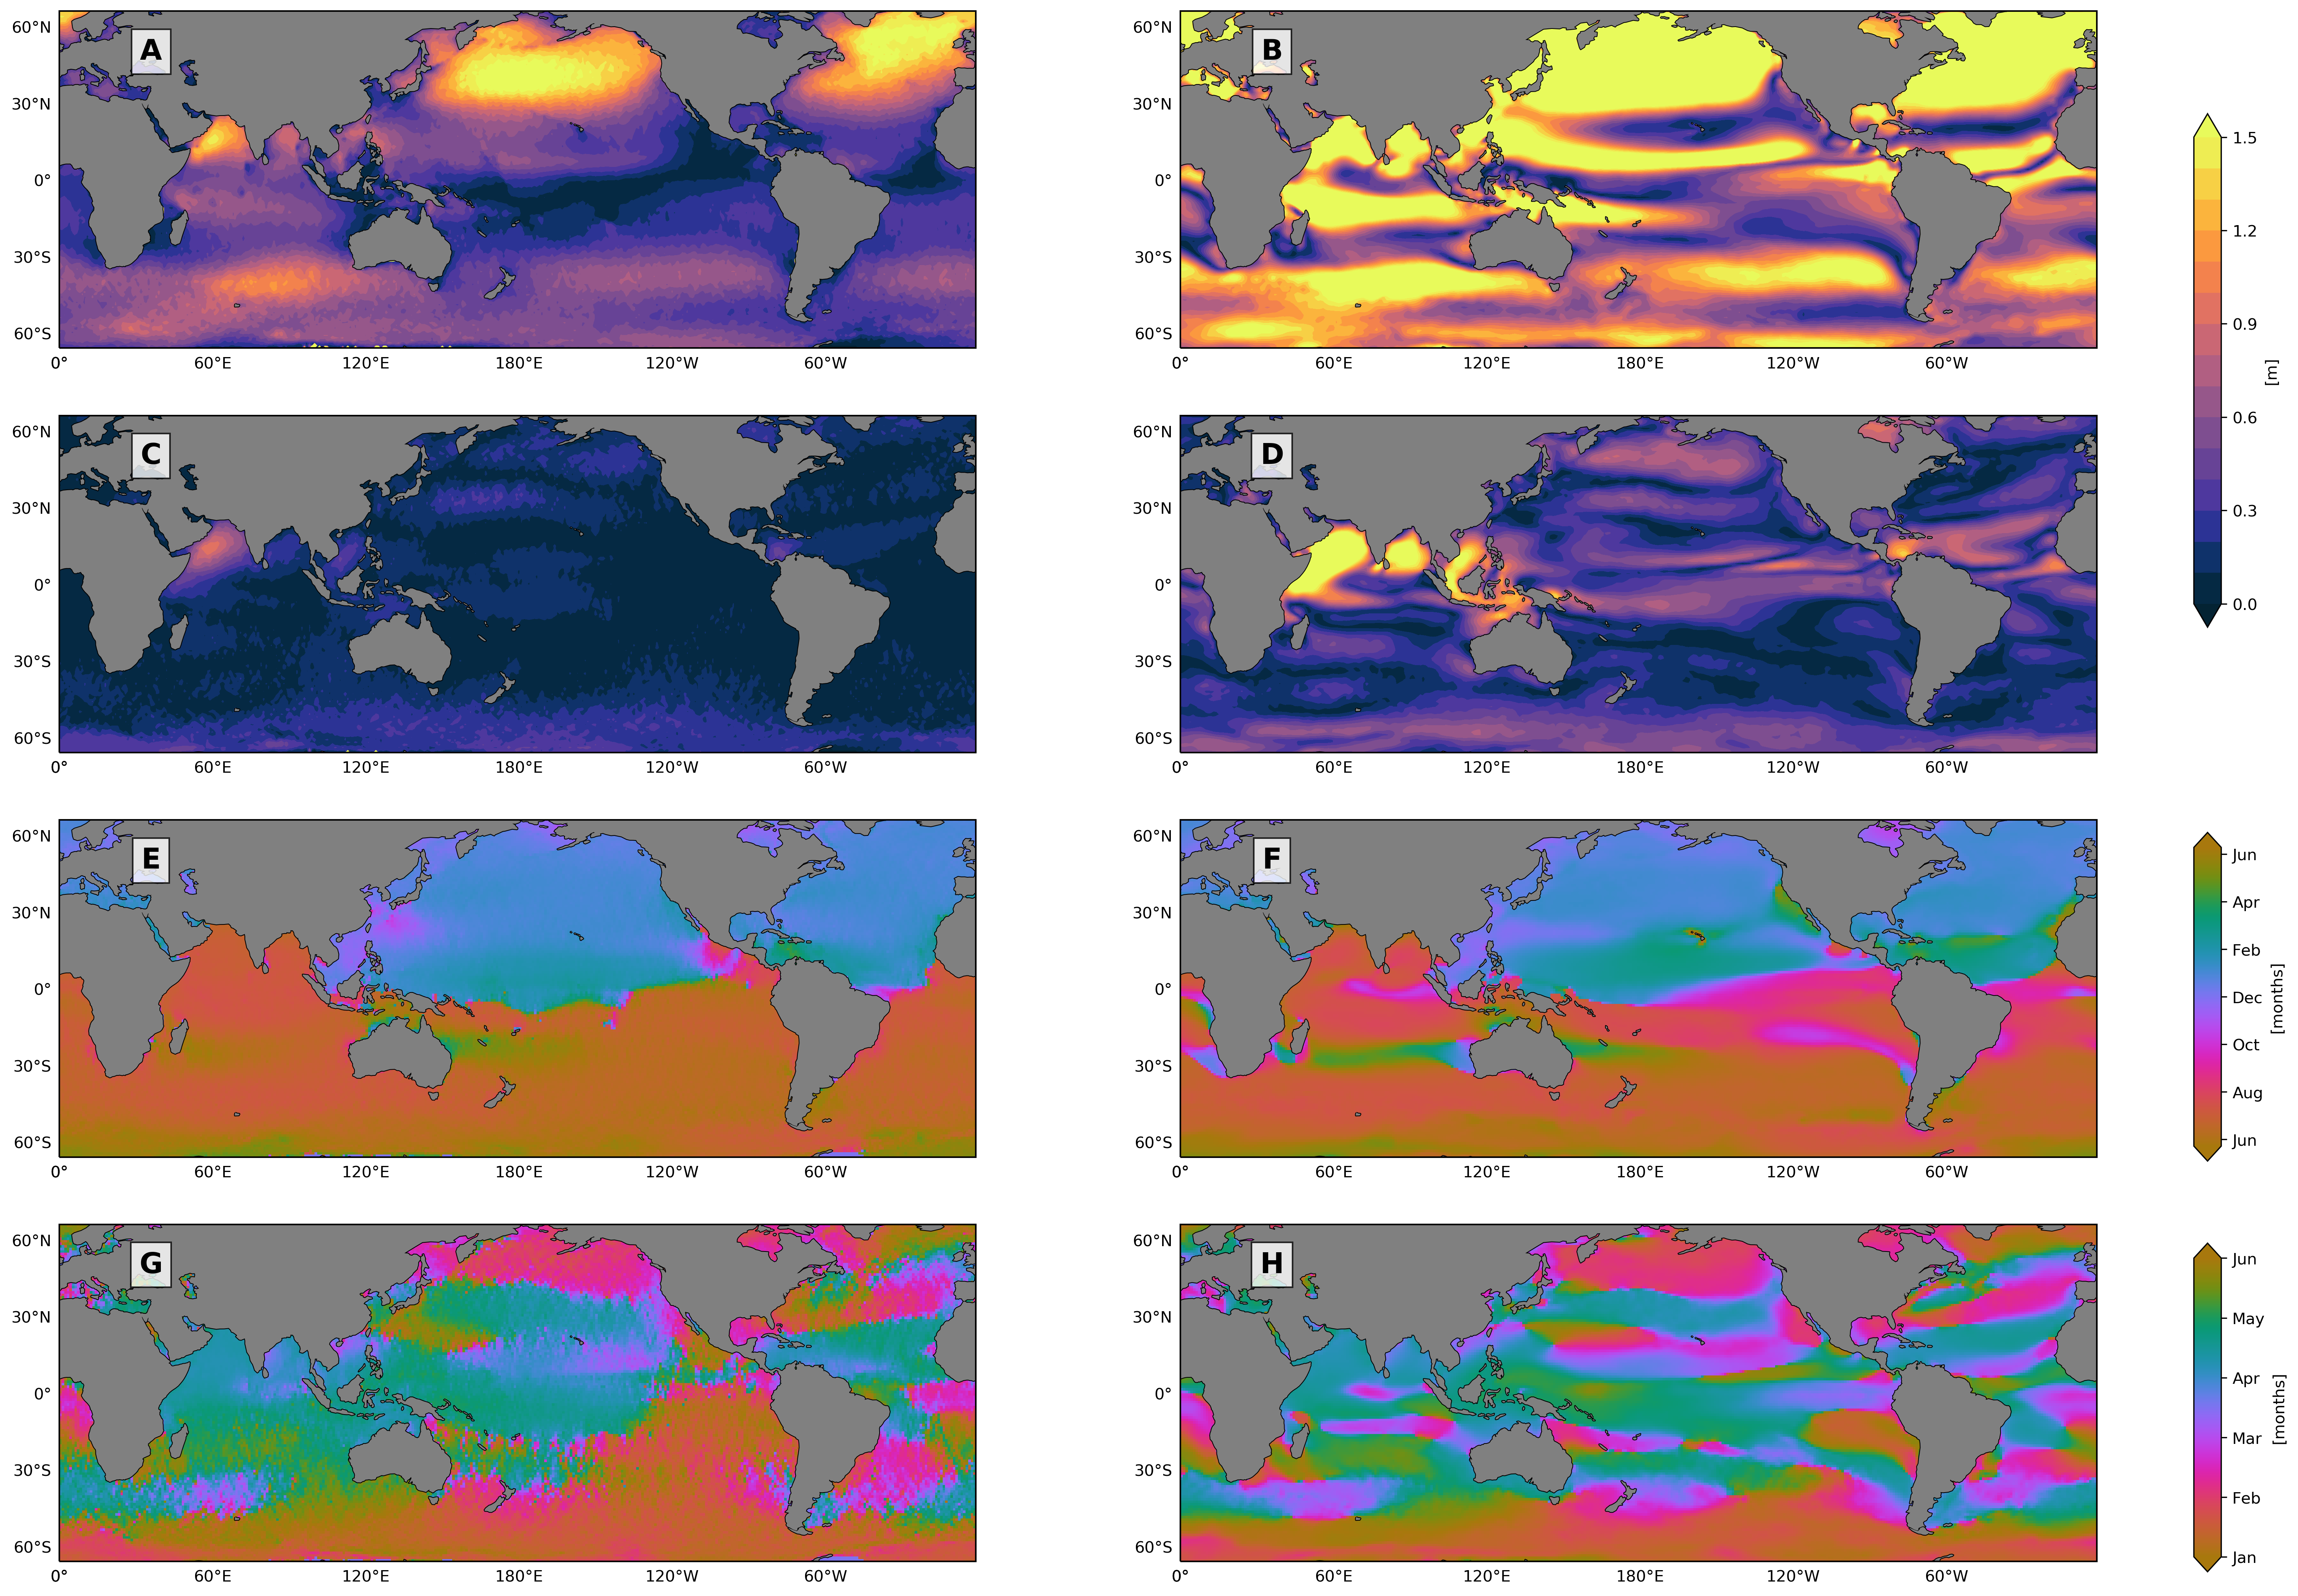
\includegraphics[width=1.0\textwidth]{figs/lsf_parameters/ccmp2_ifremer_lsf_parameters_5_par_fit_paper.png}
\caption{Amplitude of annual cycle for (A) Ifremer SWH and (B) CCMP2 WSP; amplitude of semi-annual cycle for (C) Ifremer SWH and (D) CCMP2 WSP; phase of annual cycle for (E) Ifremer SWH and (F) CCMP2 WSP; phase of semi-annual cycle for (G) Ifremer SWH and (H) CCMP2 WSP.  See text for details of computation.}
\label{Ifremer_ccmp2_lsf_chars}
\end{figure}

The annual cycle phase map for SWH (Fig.~\ref{Ifremer_ccmp2_lsf_chars}E) shows that the phase of the seasonal cycle in the Northern Hemisphere is approximately 6 months out of phase with the Southern Hemisphere, with the timing of maximum wave height well aligned with the timing of maximum WSP seasonal cycle (Fig.~\ref{Ifremer_ccmp2_lsf_chars}F). WSP is a common characteristic of these storm systems and experiences a seasonal cycle (Fig.~\ref{CCMP2_wsp_seasonal_mean}). Remotely forced waves generated from these near surface winds will propagate away from these storm systems throughout ocean basins and will predominately dominate the wave field \cite{semedo2011global}. This causes SWH of these remotely forced waves to undergo a similar seasonal cycle(Fig.~\ref{Ifremer_swh_seasonal_mean}). Therefore, this 6-month phase shift illustrates that storm systems' annual frequency and intensity cycles in the mid to high latitudes of the Northern and Southern Hemispheres set the seasonal cycle of SWH. However in some regions where local wind events input a significant amount of energy into the ocean, the wave field may become dominated by locally forced waves.

Other features in the SWH annual cycle phase map include higher spatial variability in the Southern Hemisphere than in the Northern Hemisphere, potentially due to the nontrivial wind systems present in the Southern Hemisphere experiencing high amplitude intraannual variability. The intraannual variability of storm system would directly effect the wave climate because remote and local storms or prevailing winds are one of the main forcing mechanisms generating these wind waves. Therefore, high spatial variability in phase exists in the southern hemisphere. In the equatorial region, the dominant phase changes roughly along a line where the amplitude of the seasonal cycle tends towards zero (Fig~\ref{Ifremer_ccmp2_lsf_chars}A). This boundary designates the transition from the seasonal cycle being primarily set by storm system originating in the Northern hemisphere to being primarily set by storm systems originating in the Southern Hemisphere. This smooth transition is expected in the region where the amplitude tends towards zero. This phase boundary in the Pacific and Atlantic is also known as a swell front \cite{young1999seasonal} and is the boundary between domains of dominance of swell from each hemisphere and discussed in \citet{semedo2011global} and \citet{jiang2013global}. However, waves propagating from the Northern and Southern Hemispheres coexist superimposed on the wave field at and beyond the swell front \cite{echevarria2019seasonal}. This means that the waves will continue propagating in their respective directions into the opposite hemisphere.

In the tropical Pacific, several abrupt shifts in phase exist between 10$^{\circ}$ and 20$^{\circ}$ south at approximately 180$^{\circ}$E and 145$^{\circ}$W (Figure~\ref{phase_amp_topo_comp}). One explanation for these abrupt phase shifts is island shadowing. Waves from the Southern Ocean propagating northward encounter the topography of Polynesian islands and break and dissipate on the shores facing the direction of the oncoming waves. The opposite side of the island does not encounter any of these remotely or locally forced waves. Therefore, the southern facing sides of these islands are in phase with the Southern Hemisphere seasonal cycle while the northern facing sides of the islands are in phase with the northern hemisphere because they are only exposed to southward traveling waves originating in the Northern Hemisphere. Some waves are able to squeeze between these islands as well. Waves from the Southern Ocean that are able to propagate through the Polynesian islands continue into the northern Pacific. Evidence for this northward propagation can be seen in a tongue of slightly higher phase constant value between the two indentations present on the phase boundary at approximately 175$^{\circ}$E and 140$^{\circ}$E (Figure~\ref{phase_amp_topo_comp}A). Higher phase constant value refers to the maximum of the SWH annual cycle is occurs during the spring months of May or April as it shifts towards the boreal winter. 

%In Figure~\ref{phase_topo_comp}, islands lie around these indentations and there are clear examples of island shadowing occurring at below the indentations at 180$^{\circ}$ east and 145$^{\circ}$ west. These two larger island clusters north facing shores have very little or no exposure at all to waves propagating from southern ocean storms. This cause a small region on the north facing shore to be in phase with the northern hemisphere seasonal cycle such that the region primarily exposed to northern hemisphere remotely forced waves.  

\begin{figure}[htb]
\centering
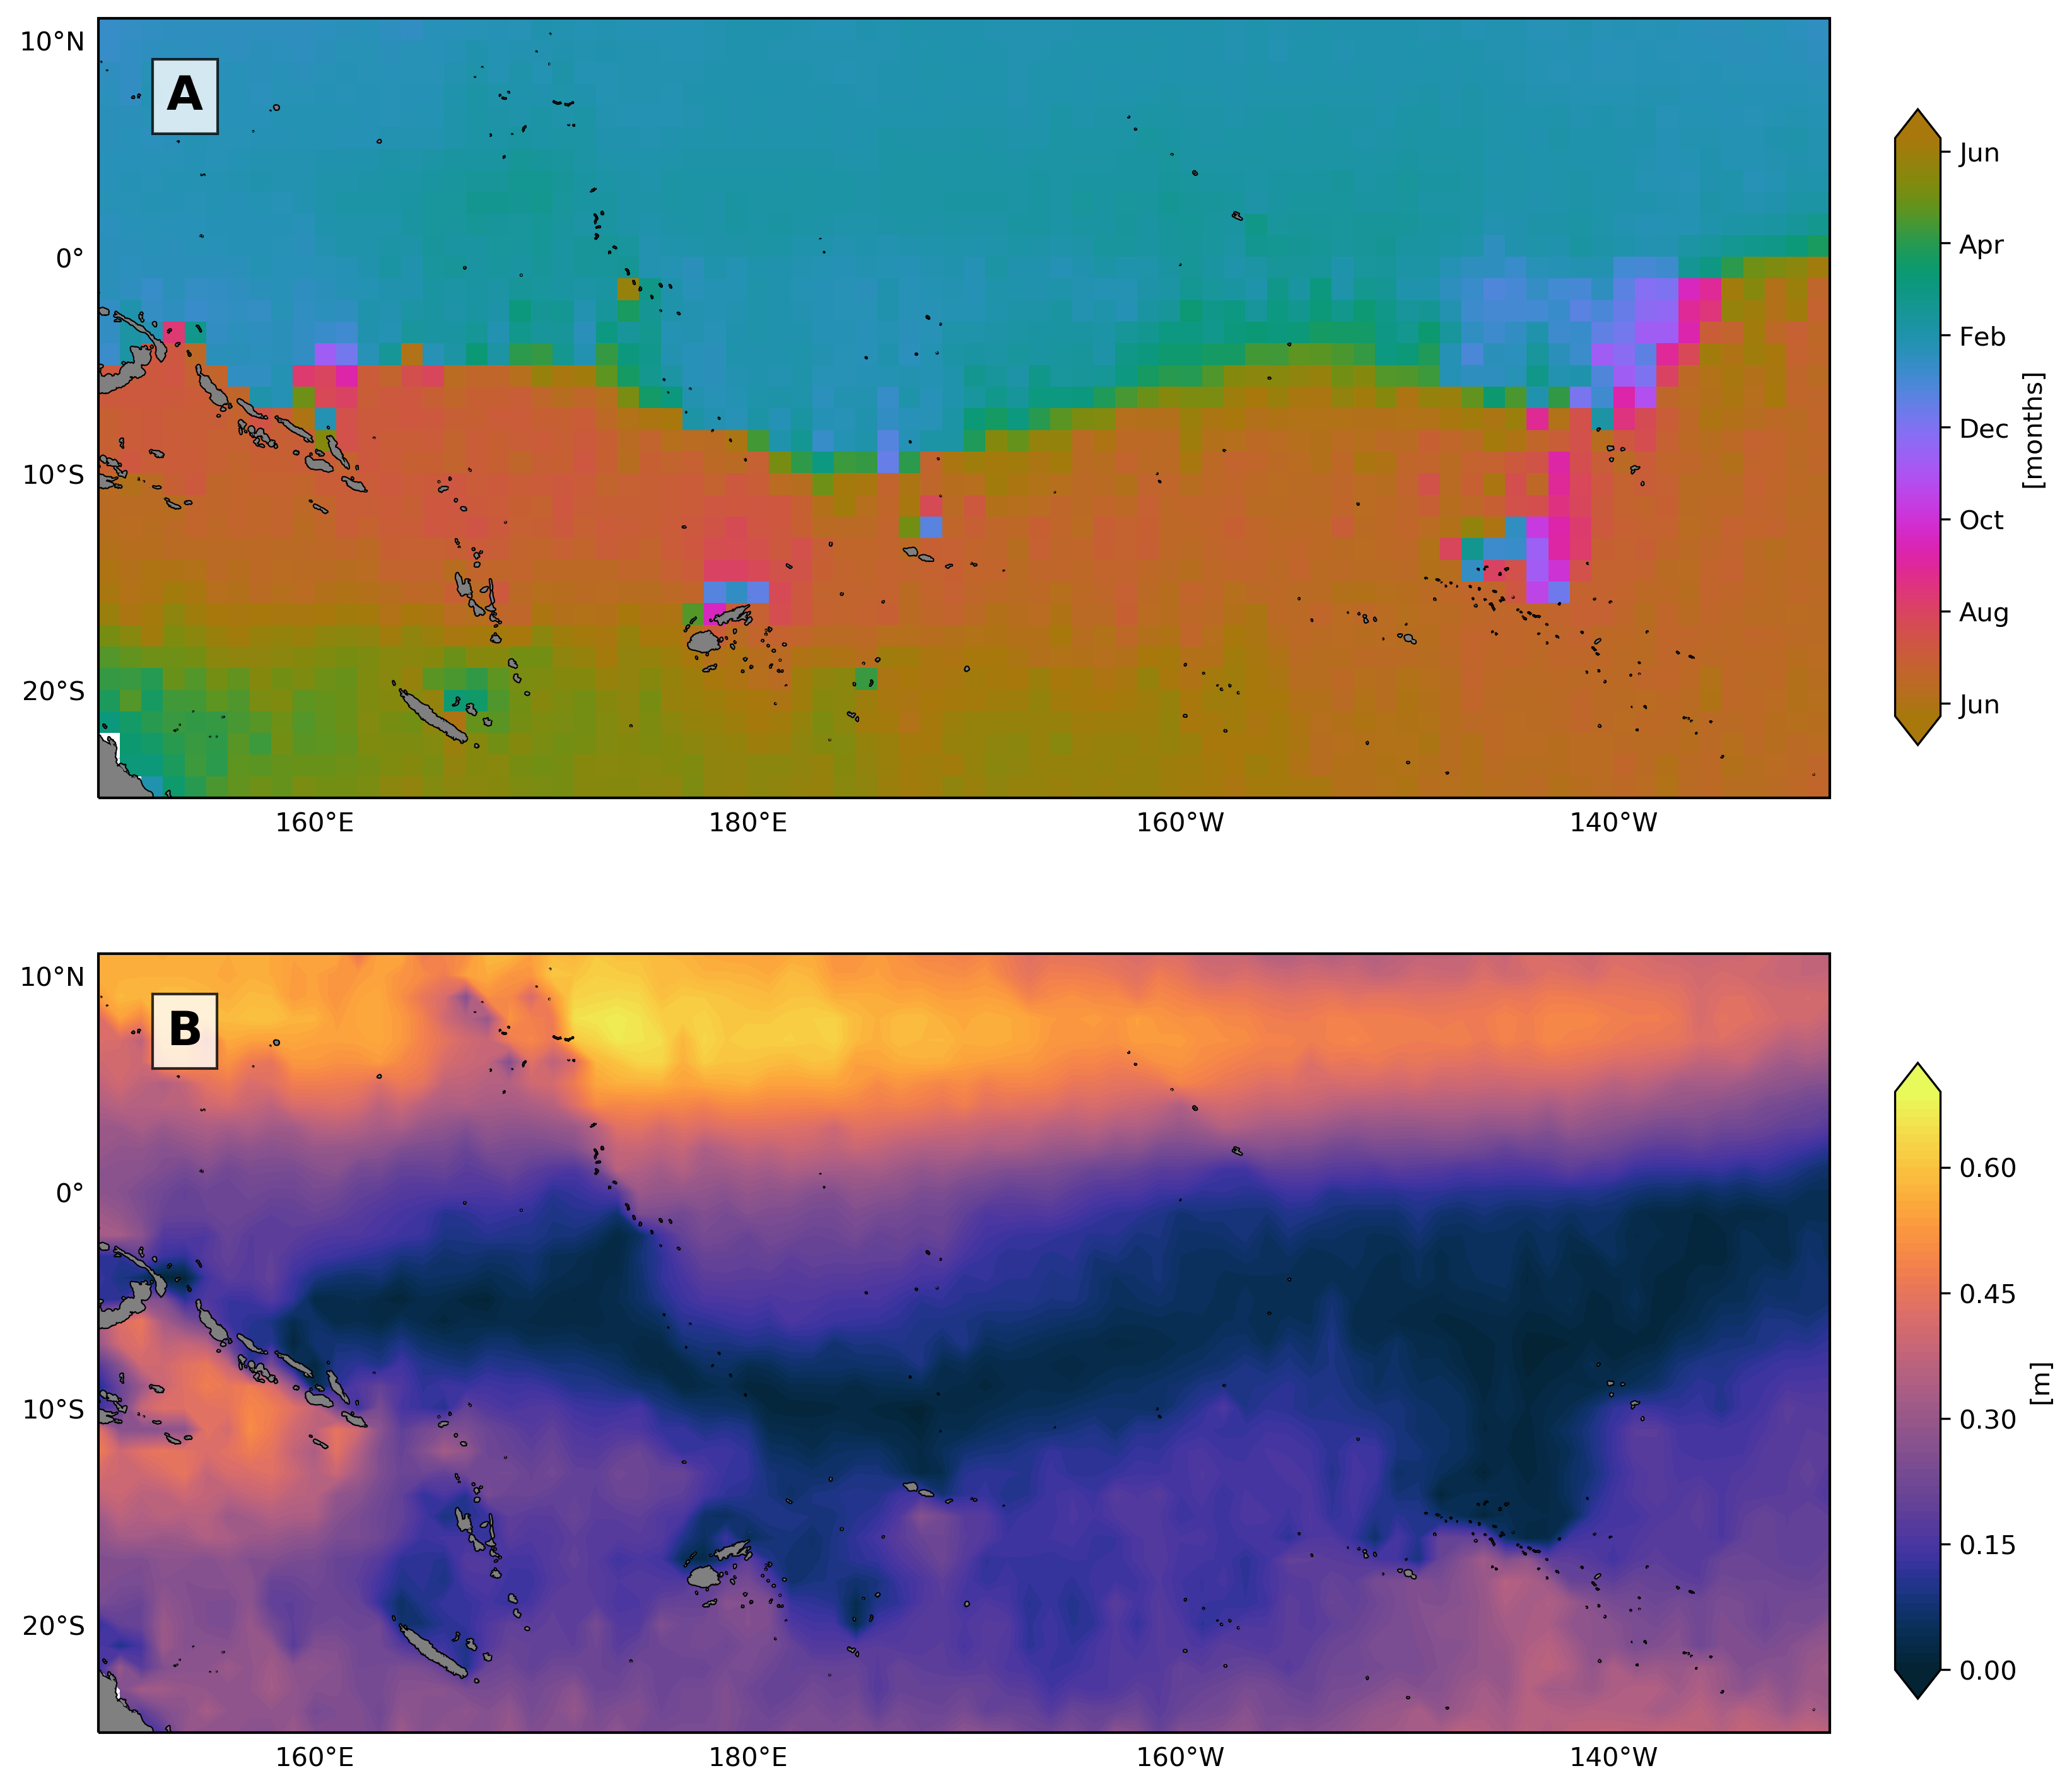
\includegraphics[width=1.0\textwidth]{figs/lsf_parameters/Phase_amp_topography_overlap.png}
\caption{(A) Ifremer SWH Annual cycle phase map in Polynesian island region illustrating island shadowing, (B) Ifremer SWH annual cycle amplitude map in Polynesian island region }
\label{phase_amp_topo_comp}
\end{figure}

The phase transition from the Northern Hemisphere dominated domain to the Southern Hemisphere dominated domain occurs slightly south of the equator between 5$^{\circ}$ and 10$^{\circ}$S in the west pacific staring at 170$^{\circ}$W , and it slowly shifts equatorward while moving east across the Pacific (Figure~\ref{phase_amp_topo_comp}A). Explanations for the geographic location of the boundary are linked to where the amplitude of the seasonal cycle tends to zero (Figure~\ref{phase_amp_topo_comp}B). Other explanations include the following. Waves would encounter westward flowing south equatorial current (SEC), south equatorial countercurrent (SECC), the westward north equatorial current (NEC), or the north equatorial countercurrent (NECC). The SEC and SECC are located on average closest to the phase boundary, and they are known to be present between 5$^{\circ}$ and 10 $^{\circ}$S \cite{talley2011descriptive}. However, the wave-current interactions between waves propagating into this region from the Northern and Southern Hemisphere have no effects of wave propagation when the velocities of the two are orthogonal. In addition, the wave-current interaction is on small scales and would be undetectable in satellite altimeter SWH data when the footprint of the satellite covers several kilometers of sea surface. Additionally, the phase boundary of the annual cycle does not line up with the intertropical convergence zone (ITCZ) characterized as a low pressure system with heavy precipitation and deep convection \cite{schneider2014migrations} that causes very calm sea surface conditions. These calm sea surface conditions could be thought of as being associated with the low amplitude seasonal cycle region. However, low amplitude does not imply low SWH values because there is a mean value that offsets the SWH seasonal oscillations from zero. By looking at the SWH seasonal mean (Fig~\ref{Ifremer_swh_seasonal_mean}), the mean is relatively low, but not the minimum value of the equatorial region. In addition, the intertropical convergence zone annual migrates between 9$^{\circ}$N in boreal summer and 2$^{\circ}$N in boreal winter in the central Pacific following the warmer hemisphere \cite{schneider2014migrations}. This is significantly far from the phase boundary. Wave to wave interactions and non-conservative forcing could possible play a significant role here; however, the angle between each wave's group velocity determines significantly how energy and momentum will be distributed throughout the system. By looking at fig~\ref{phase_amp_topo_comp}, we see that islands within this region play a significant role in setting the shape of the minimum annual cycle amplitude region for SWH. Islands outline the near zero contour for amplitude and therefore significantly affect how waves propagate into this region and how those waves will interact with each other. 

Other interesting structures exist in near coastal regions and in the Atlantic in Fig.~\ref{Ifremer_ccmp2_lsf_chars}E. In the Atlantic, there is also a smooth phase boundary transition with one abrupt phase shift close to the western side of the Atlantic. On the western side, the phase boundary is almost vertical following a line of constant latitude. This dynamic boundary also occurs in the zero amplitude SWH seasonal cycle region and is slightly below the equator. In addition, just off the coast of Mexico, there is an out of phase region that is close to the near zero amplitude region. These other structures will be left for further research.

\begin{figure}[tbh]
\centering
  \begin{minipage}{.5\textwidth}
    \centering
    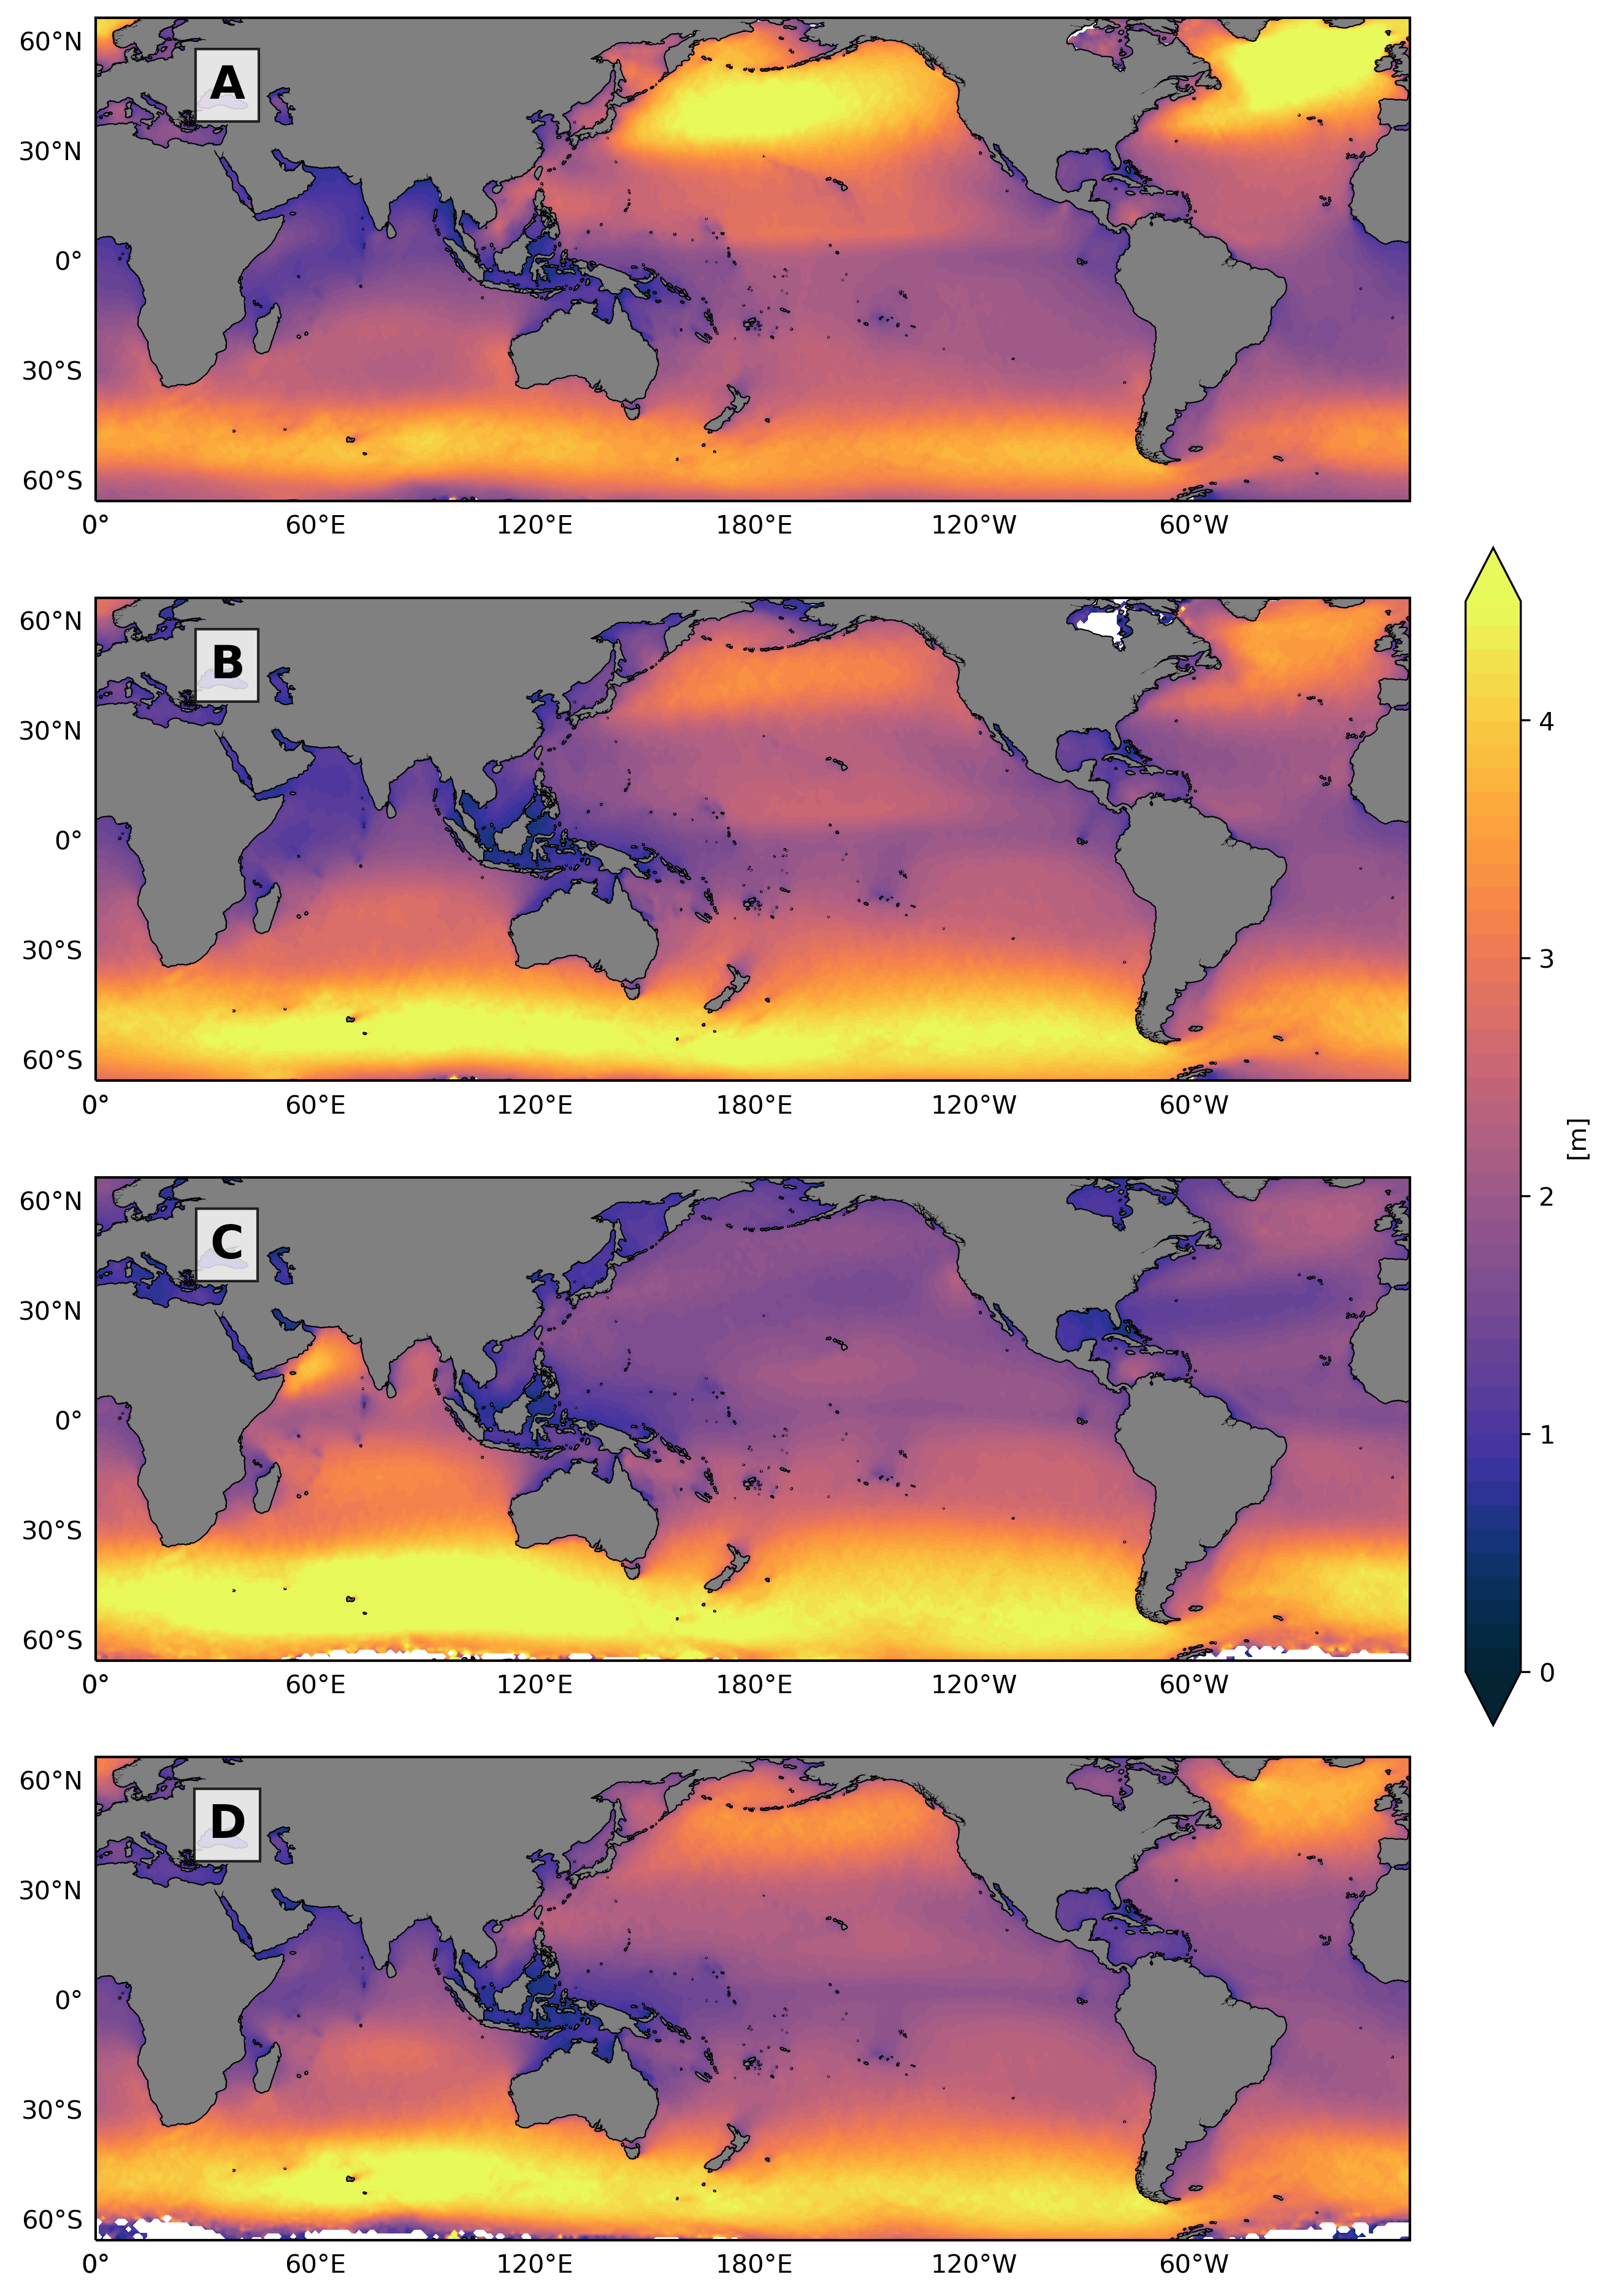
\includegraphics[width=0.5\textwidth]{figs/statistical_moments/Ifremer_p1_seasonal_mean.png}
    \caption{Ifremer SWH Seasonal Mean}
    \label{Ifremer_swh_seasonal_mean}
  \end{minipage}%
  \begin{minipage}{.5\textwidth}
    \centering
    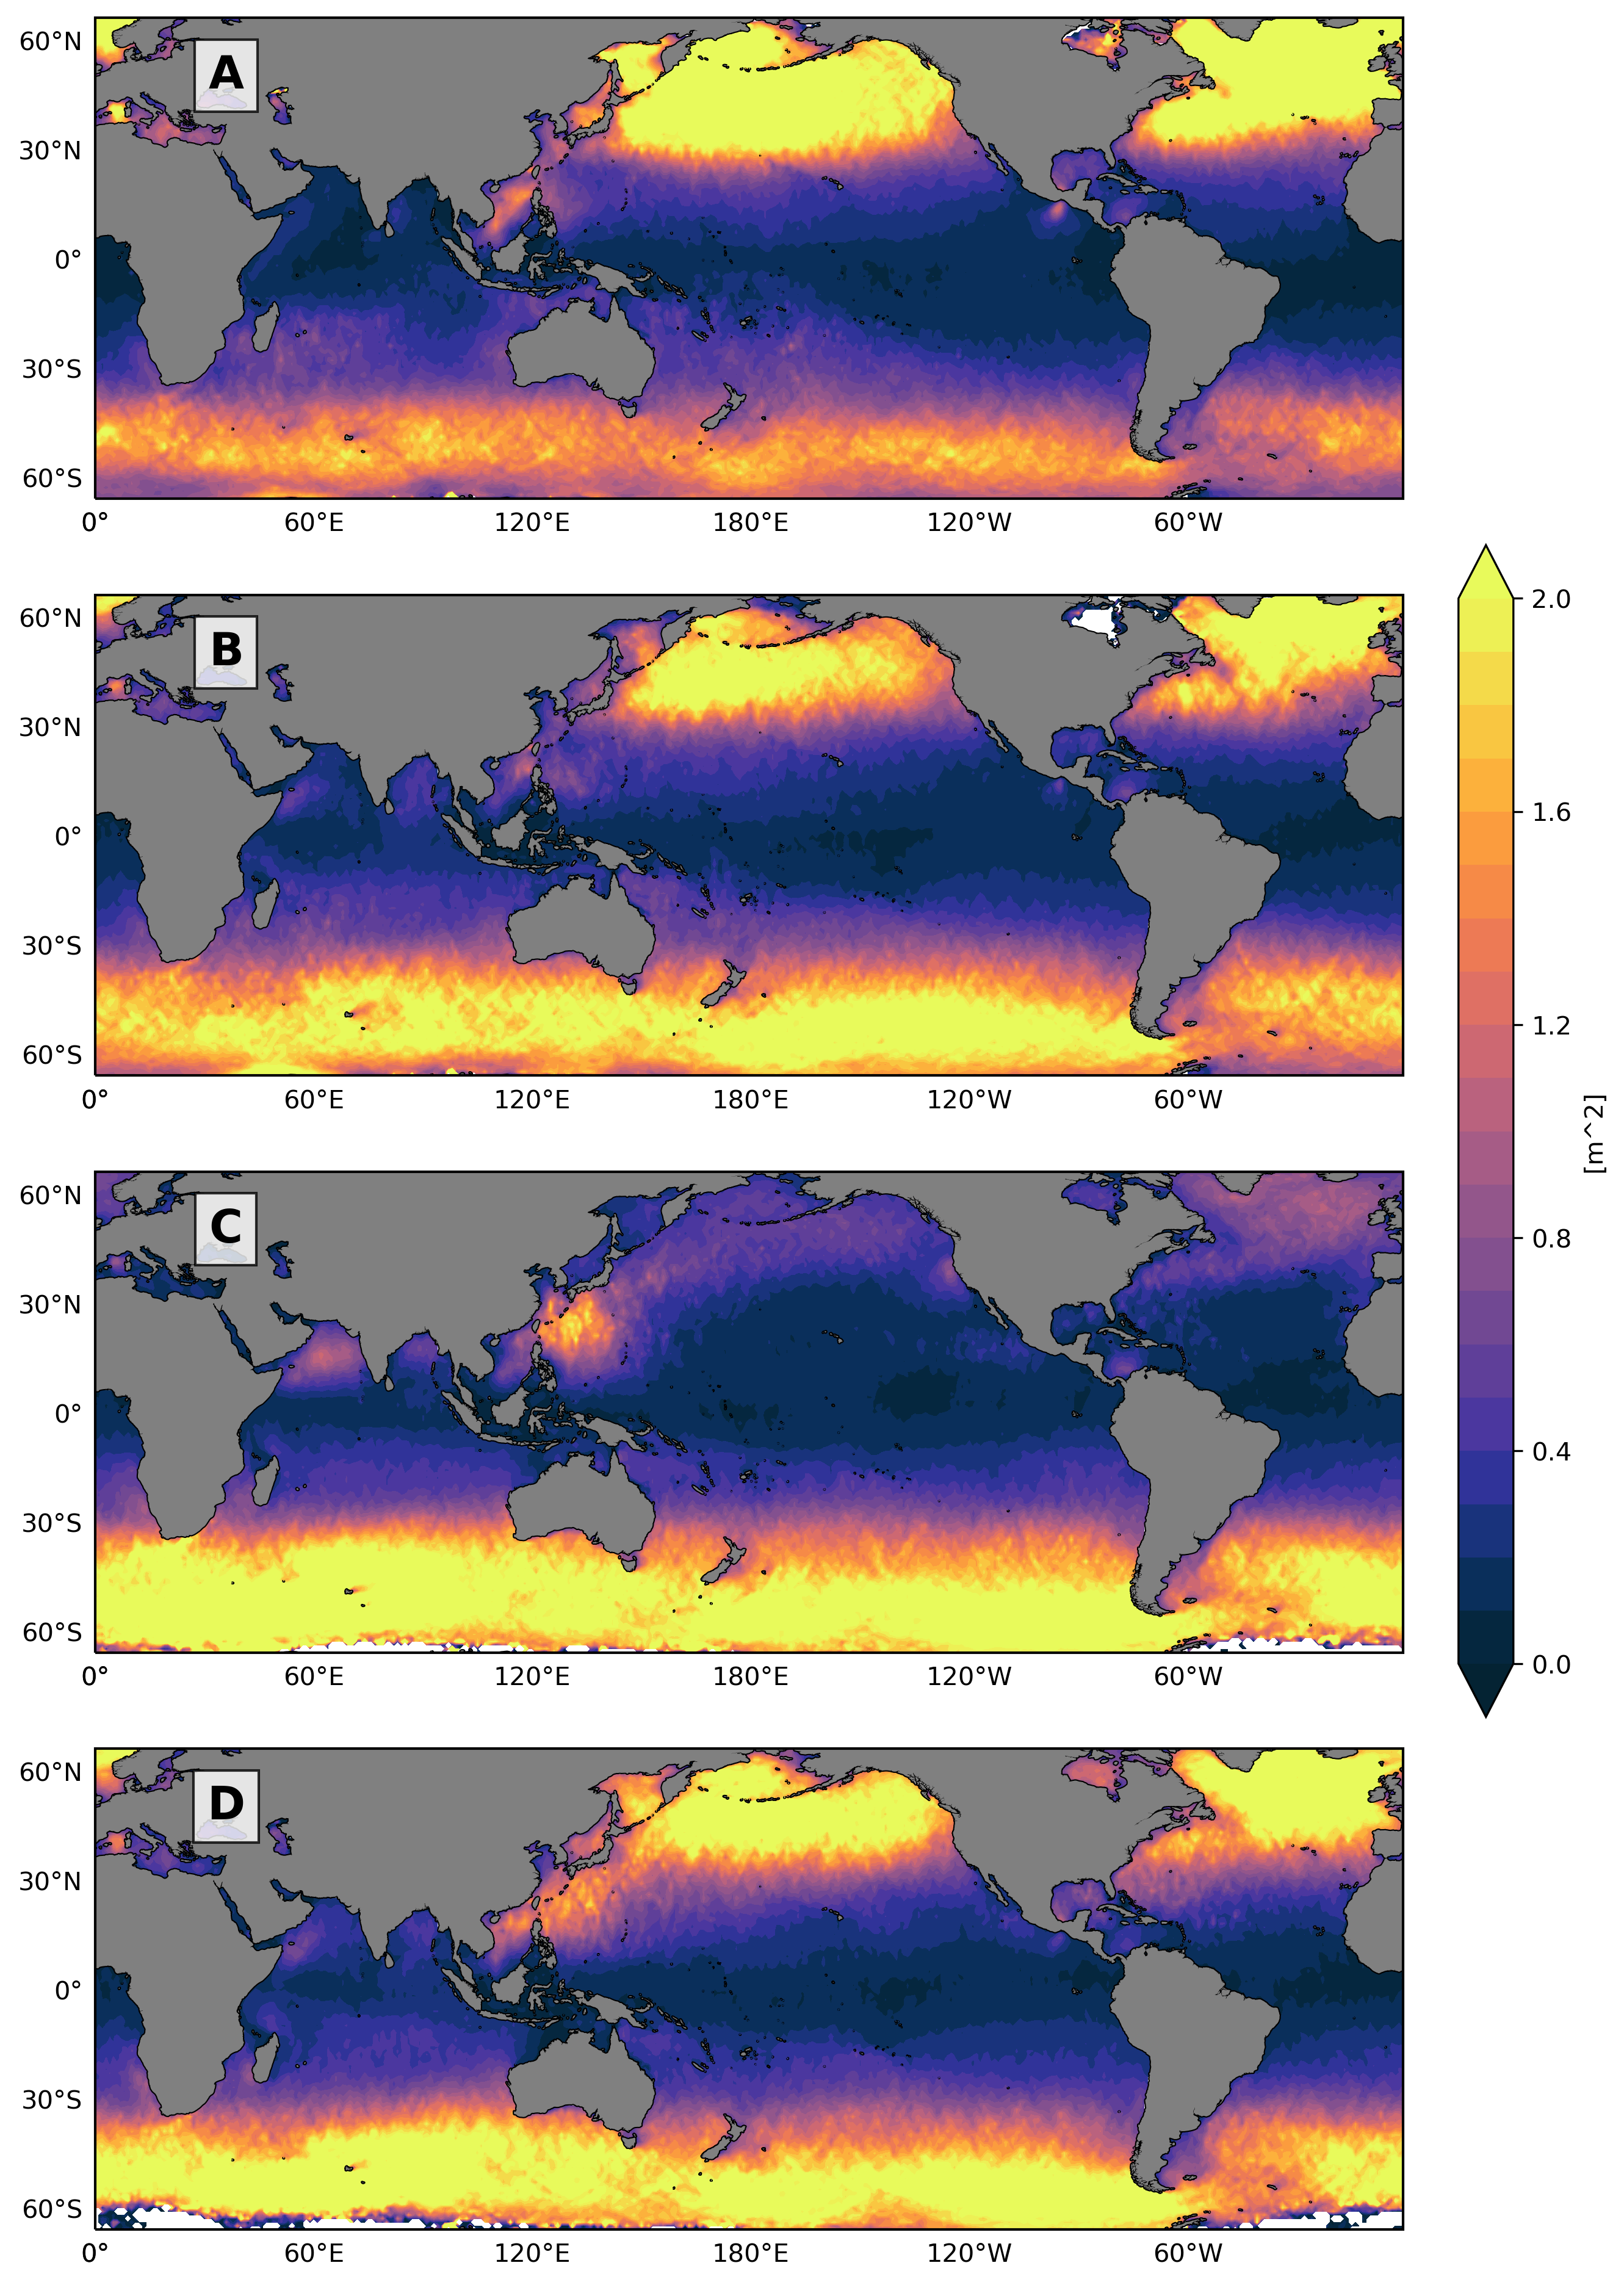
\includegraphics[width=0.5\textwidth]{figs/statistical_moments/Ifremer_p1_seasonal_var.png}
    \caption{Ifremer SWH Seasonal Variance}
    \label{Ifremer_swh_seasonal_var}
\end{minipage}
%\caption{Ifremer SWH First and Second Statistical Moments seasonal progression with A) December through February, B) March through May, C) June %through August, and D) September through November}
\label{Ifremer_swh_seasonal_pro}
\end{figure}

\begin{figure}[tbh]
  \begin{minipage}{.5\textwidth}
    \centering
    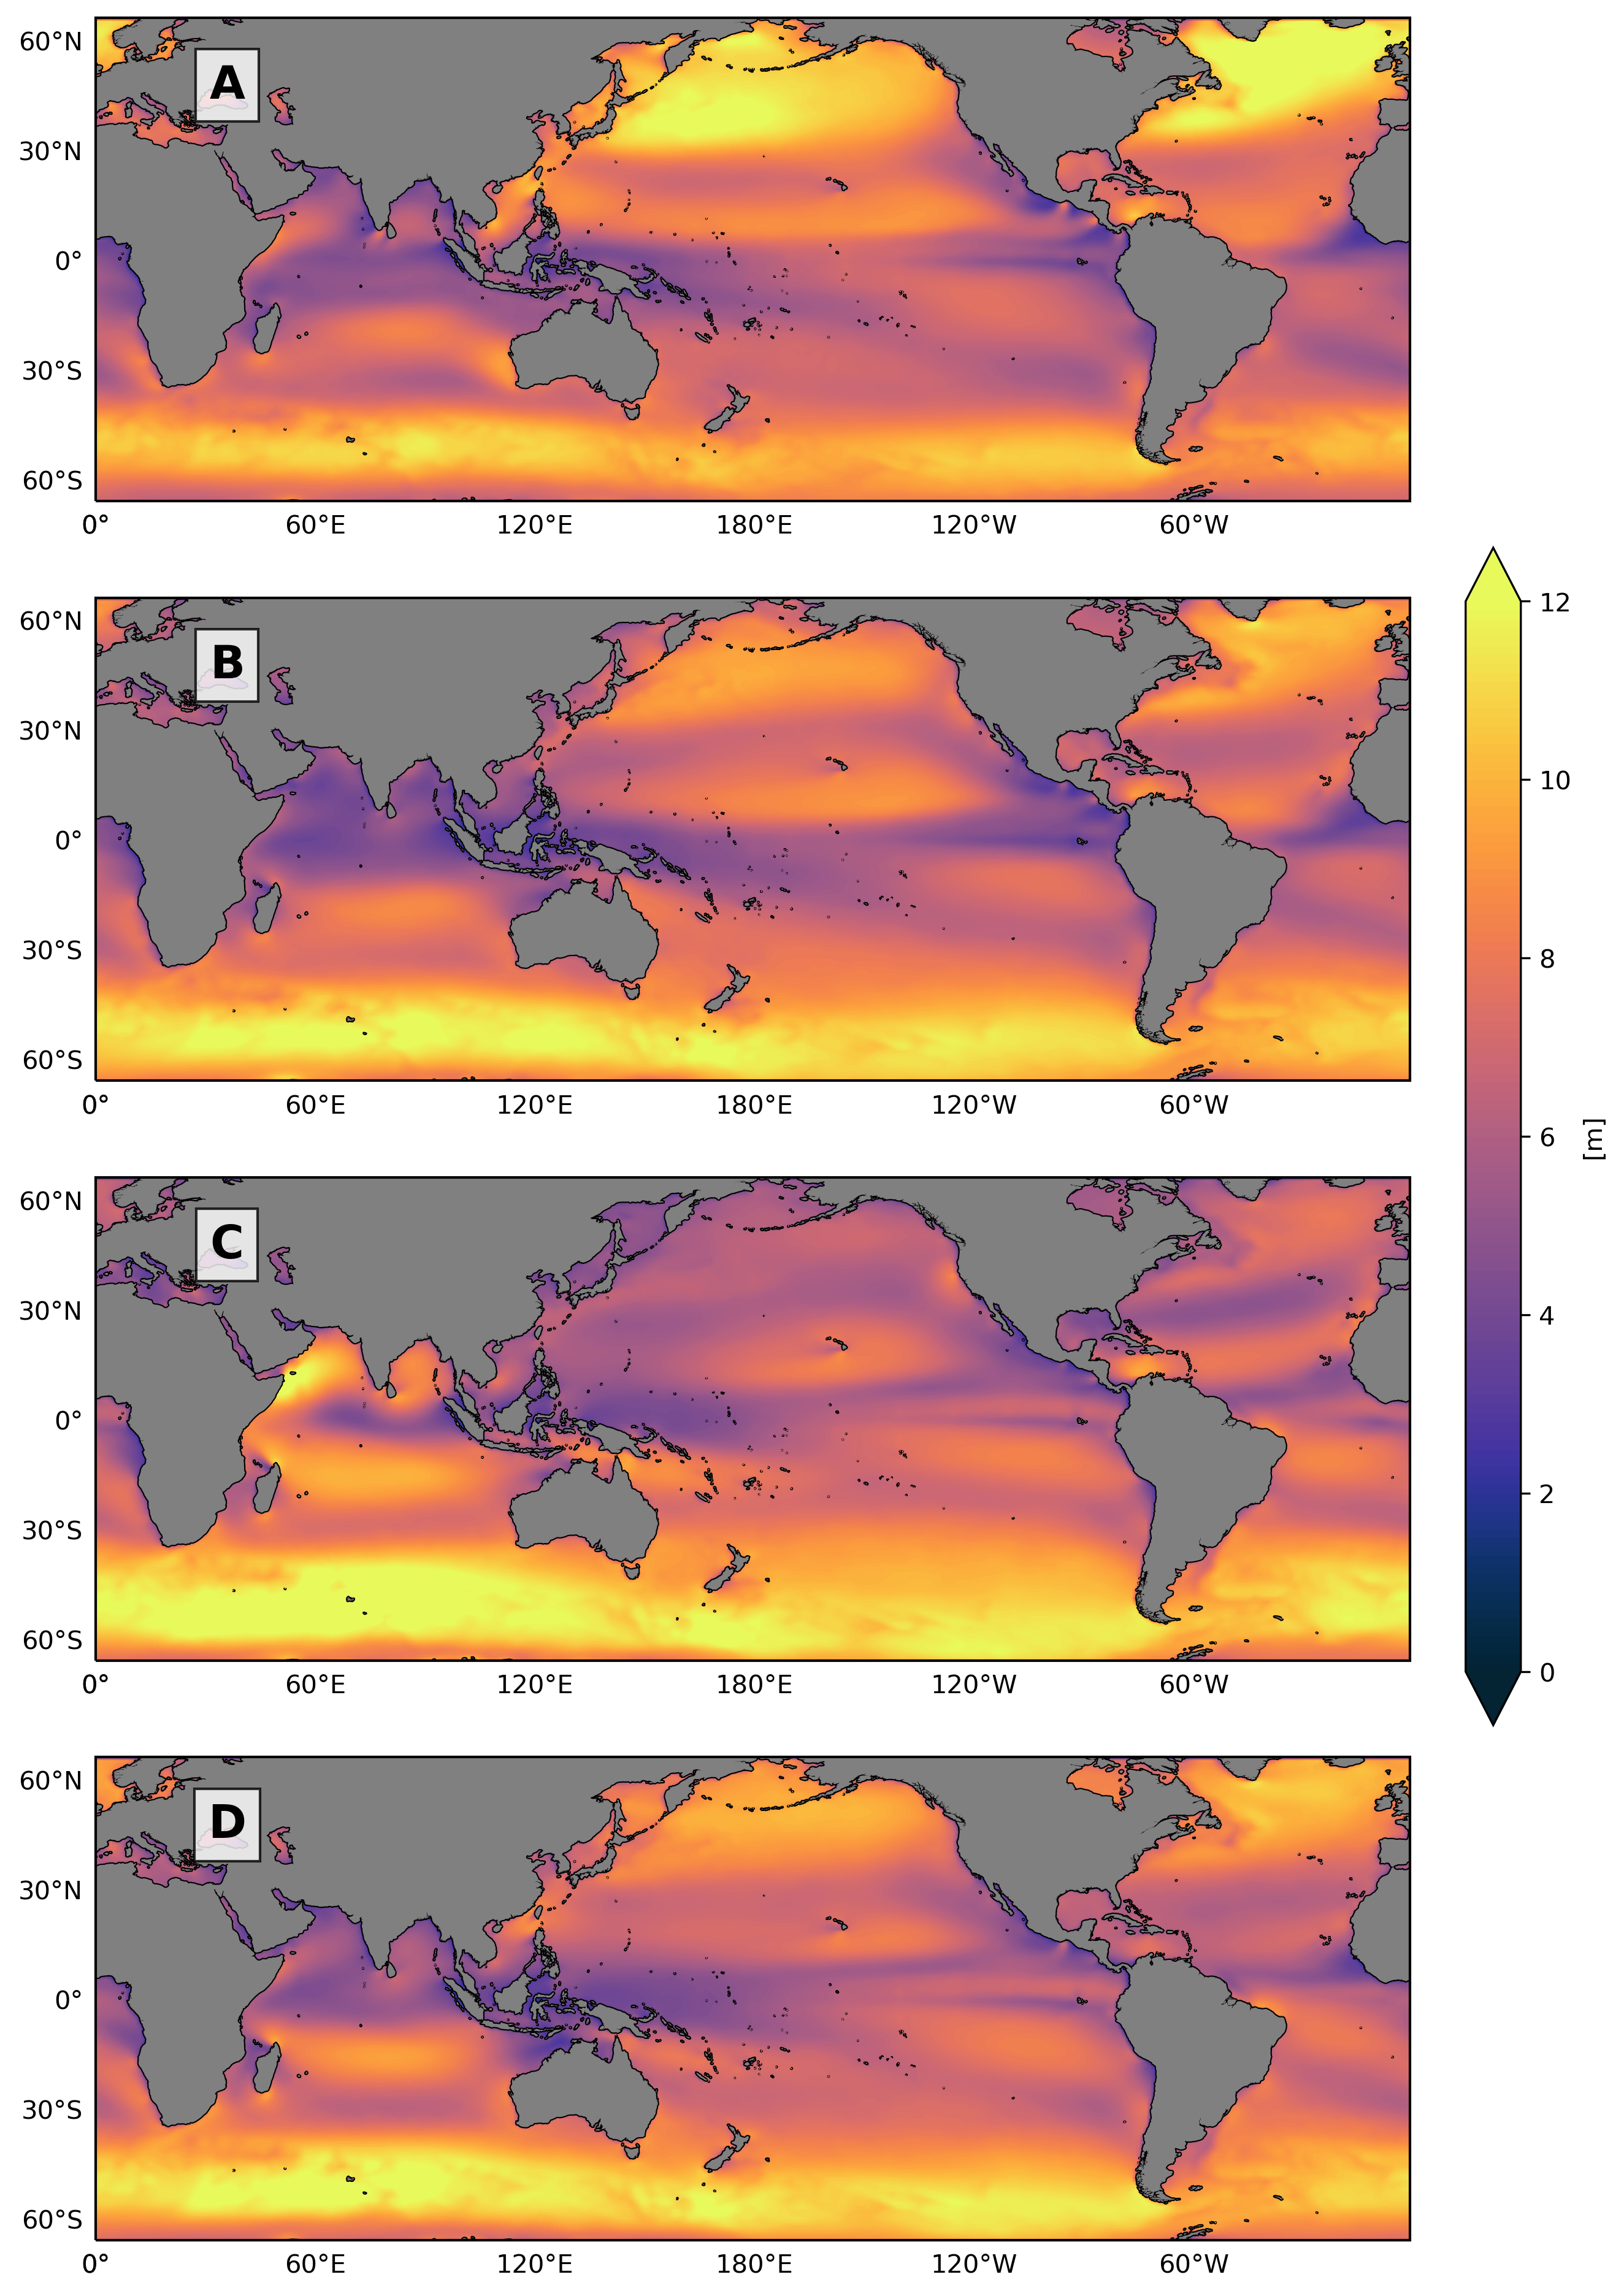
\includegraphics[width=0.5\textwidth]{figs/statistical_moments/CCMP2_seasonal_mean_wsp.png}
    \caption{CCMP2 WSP Seasonal Mean}
    \label{CCMP2_wsp_seasonal_mean}
  \end{minipage}
  %
  \begin{minipage}{.5\textwidth}
    \centering
    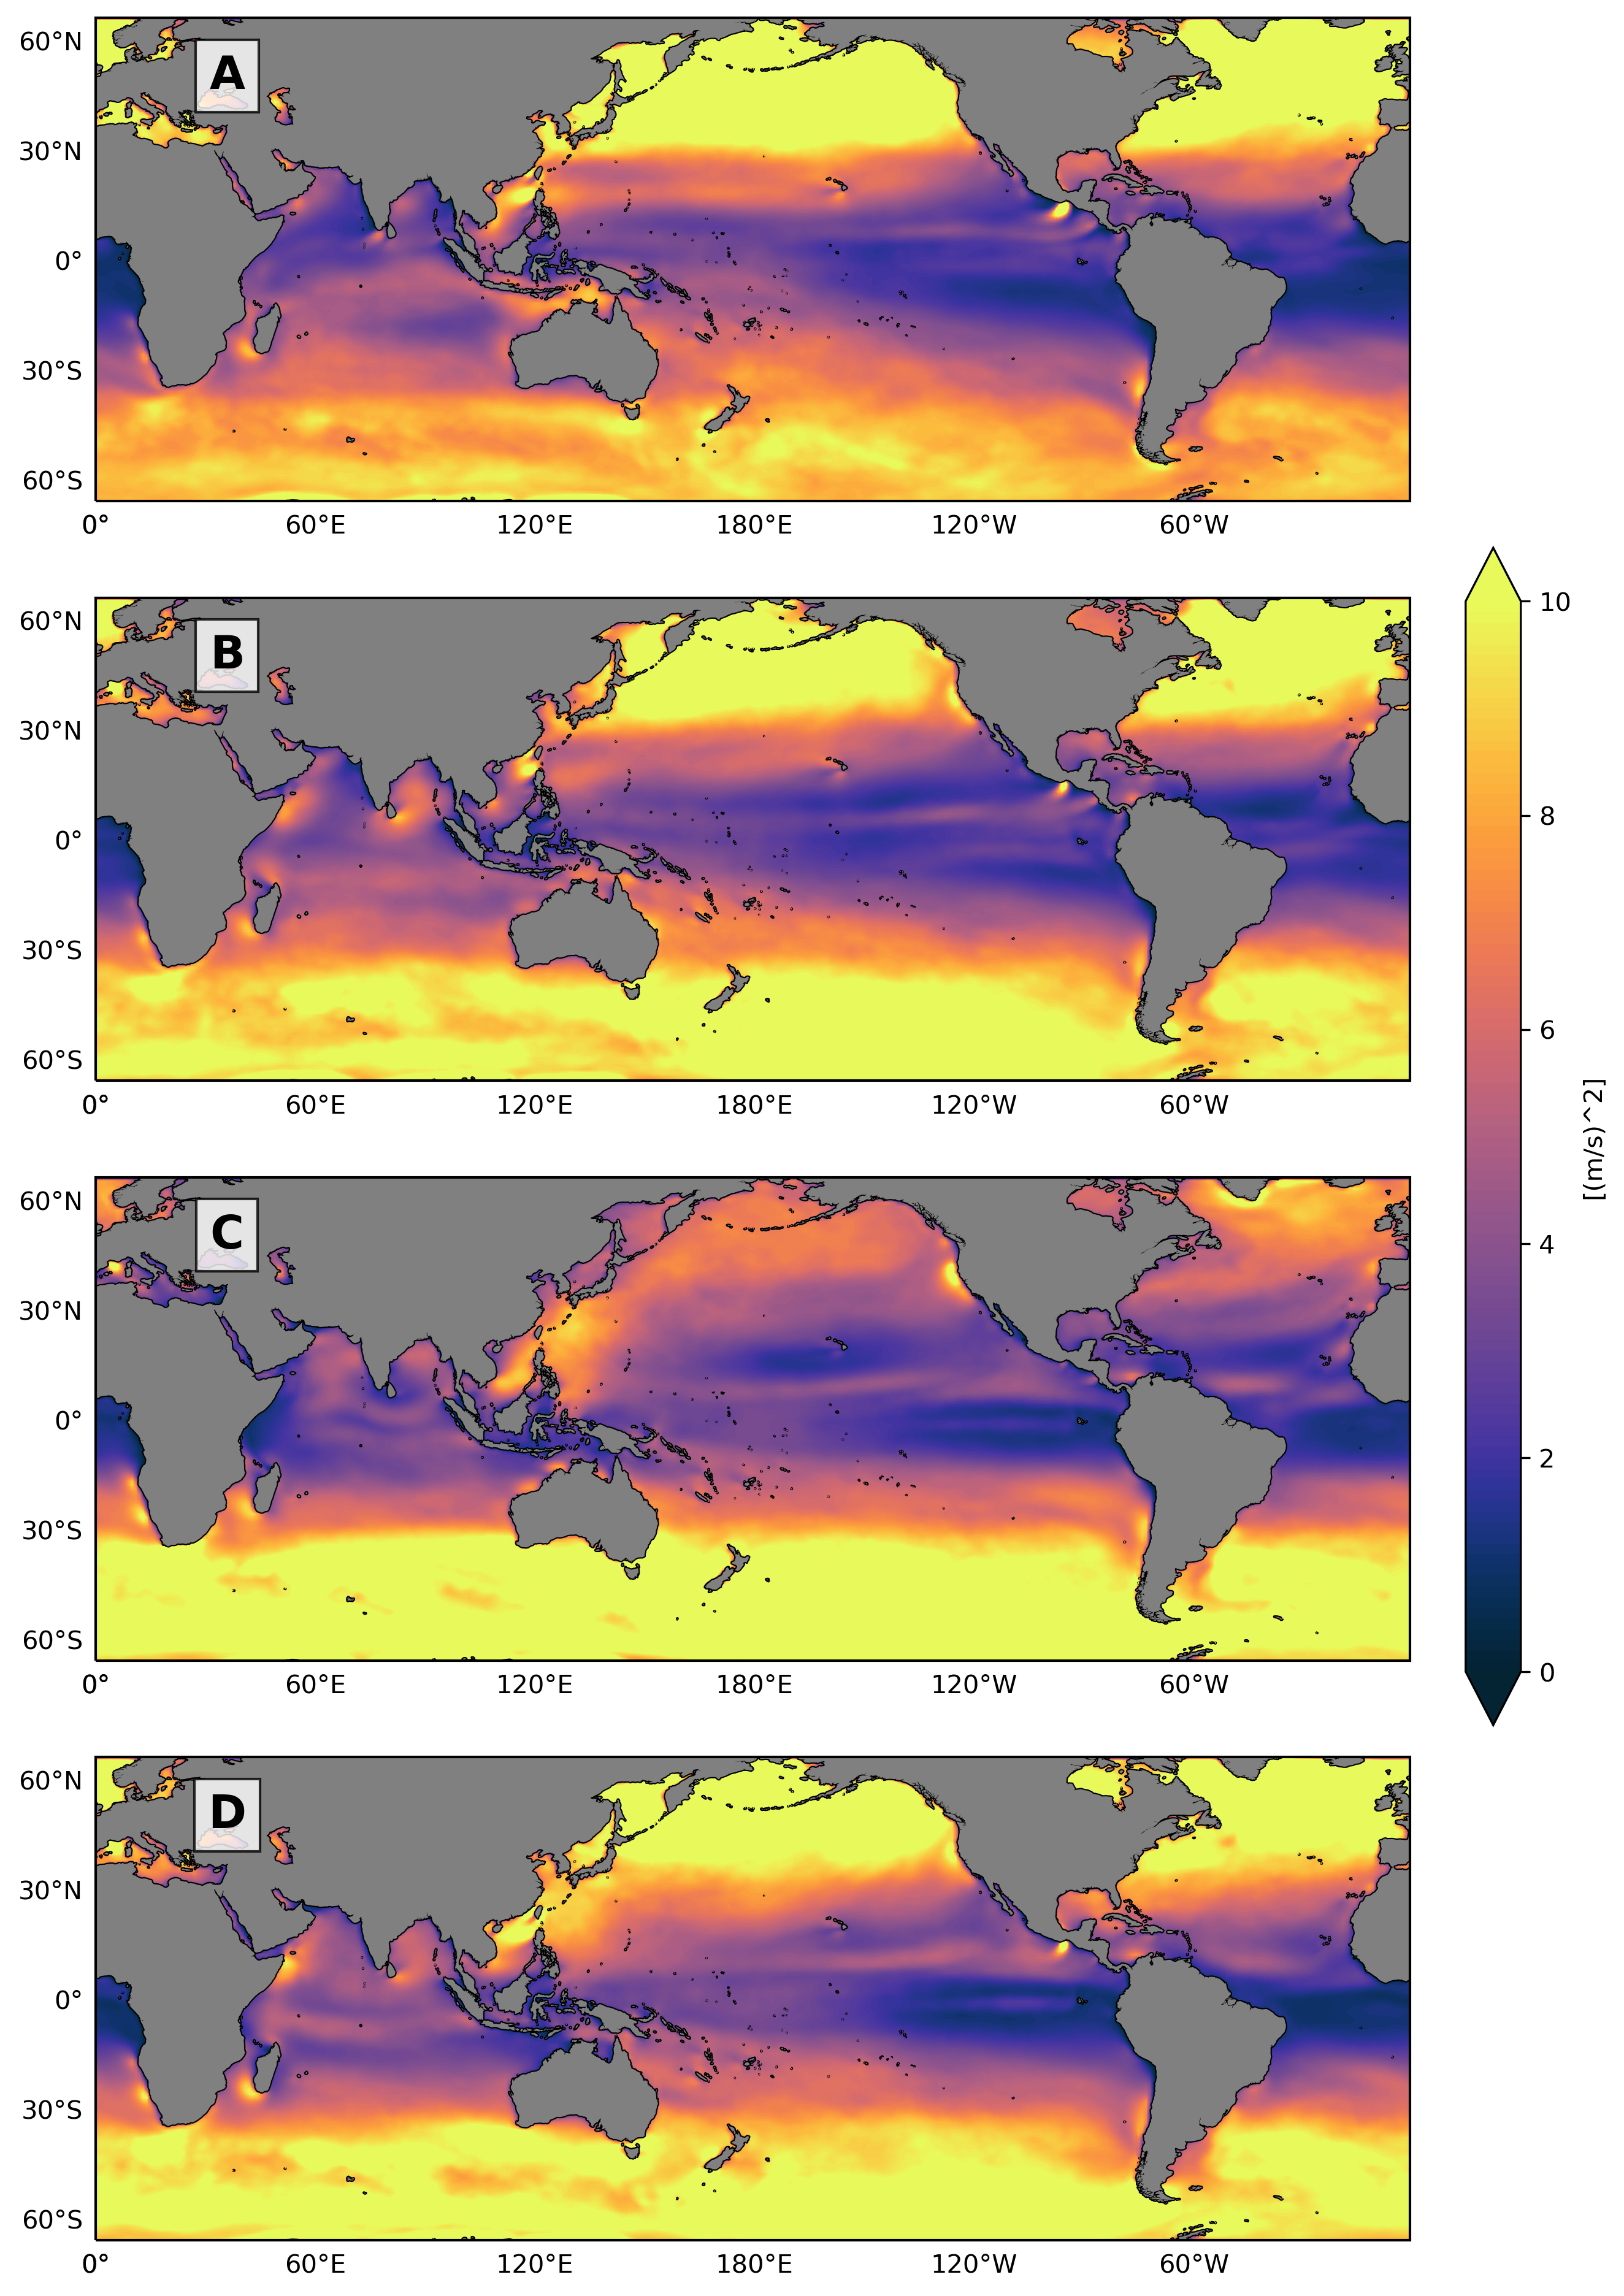
\includegraphics[width=0.5\textwidth]{figs/statistical_moments/CCMP2_seasonal_var_wsp.png}
    \caption{CCMP2 WSP Seasonal Variance}
    \label{CCMP2_wsp_seasonal_var}
  \end{minipage}
%\caption{CCMP2 WSP First and Second Statistical Moments seasonal progression with A) December through February, B) March through May, C) June through August, and D) September through November}
\label{ccmp2_wsp_seasonal_pro}
\end{figure}

The SWH and WSP annual cycle phase maps display an interesting relationship between deviations in the SWH seasonal cycle and local wind anomalies that are generated by similar mechanics to expansion fan wind events off the California coast. In the SWH annual phase constant maps, deviations from the seasonal cycle predominantly cannot be observed in the cases when the deviation in the seasonal cycle is less than the maximum values of the seasonal sinusoidal oscillations. However, this is not the case for all SWA regions, as will be explained later.  

For the WSP annual cycle phase map (Fig.~\ref{Ifremer_ccmp2_lsf_chars}F), the phase constant clearly outlines regions where local wind anomalies similar to the EFW events off the coast of California are present. The wind anomalies are characterized on the phase map by a $\pi$ phase shift in the WSP seasonal cycle or a 6 month shift is the WSP seasonal cycle maximum from the surrounding region. By looking at the global map of phase for WSP, we observe that SWA regions typically are out of phase with their surrounding regions. For example, in the EBR off the coast of Australia (Fig~\ref{Ifremer_ccmp2_lsf_chars}F), the phase reveals that the maximum in the WSP seasonal cycle occurs during the austral summer within the SWA region. Outside of the SWA region, WSP reaches a maximum during the austral winter. 

The WSP phase map has structural similarities to the SWH phase map due to the proportional relationship between wind waves and the storm systems that generate them: the Northern and Southern Hemispheres are six months out of phase with each other, and the Southern Hemisphere has more spatial variability (Fig~\ref{Ifremer_ccmp2_lsf_chars}F). These intricate Southern Hemisphere features are due to the dynamic intraannual variability of storm systems especially in the Indian ocean \cite{schott2009indian}. However, there are many differences between SWH and WSP phase maps. The phase boundary in the Pacific designating the transition in the hemisphere that is primarily setting the WSP seasonal cycle is further north, and the majority of the boundary is smooth and continuous, without abrupt changes in phase on the eastern side of the Pacific, but with a slightly high gradient on the west side. In the Atlantic, the phase boundary is a smooth transition and is more linear in shape than the SWH phase boundary in the Atlantic. The phase boundary in the Atlantic follows closely the near zero WSP amplitude of the annual cycle; however, in the Pacific, the amplitude does not tend to zero near or at the equator. Furthermore, the Indian Ocean has prominent structures of swooping fingers of high phase constant values which are again due to dynamics of intraannual variability of storm system and prevailing winds \cite{schott2009indian}. 

Coefficient of determination global maps can be used to assess the percentage of the variability explained by the model in order to understand whether there are other processes not accounted for by the annual and semi-annual cycles. Fig~\ref{Ifremer_ccmp2_lsf_gof} shows that the percent of variability explained by the model is high in the North Pacific and Atlantic and low in the Southern Ocean for SWH and WSP. For SWH, the percent variation explained reaches a minimum in the near-equatorial region in the Pacific and Atlantic. For WSP, the features of high percent variation explained are complex throughout the equatorial region with varying amounts from near 100\% to near 0\%. These low values in the equatorial region may be attributed partly to the decadal oscillation of El Ni\~no. The percent variation varies for each SWA region. For both SWH and WSP, SWA regions range from having 10\% to 40\% of the variation explained by the two modes represented in the model with the exception of the Arabian and Caribbean seas which have near 100\% variation explained. There are especially low values off the coast of Chile and Namibia for SWH and off the coasts of California, Chile, and North Africa for WSP. The Arabian and South Caribbean seas have higher percent variation explained by the model because these regions primarily have wave and wind forced by mechanics that have annual and semi-annual frequencies. In support of this argument, both of the coefficient of determinations geographic features follow very closely with features in the annual and semi-annual amplitude of SWH and WSP maps such that the percent of variation explained by the model is highest in regions with high amplitude and lowest in region of near zero amplitude. This means that the model explains the variability significantly less in most of the SWA regions because there are weak annual and semi-annual cycles. In addition, there are other forcing mechanism at work in these regions that contribute more significantly to the wave and wind field. One of these forcing mechanisms for the wave field is the deviation from the seasonal cycle from local wind events. The goodness of fit quantified by the coefficient of determination should not be thought of as a test of reliability of the model. Rather, it is an indication of physical processes not accounted for by the model, which we want to explore to understand the underlying mechanisms generating the variability in the wave and wind fields. 

\begin{figure}[tbh]
\centering
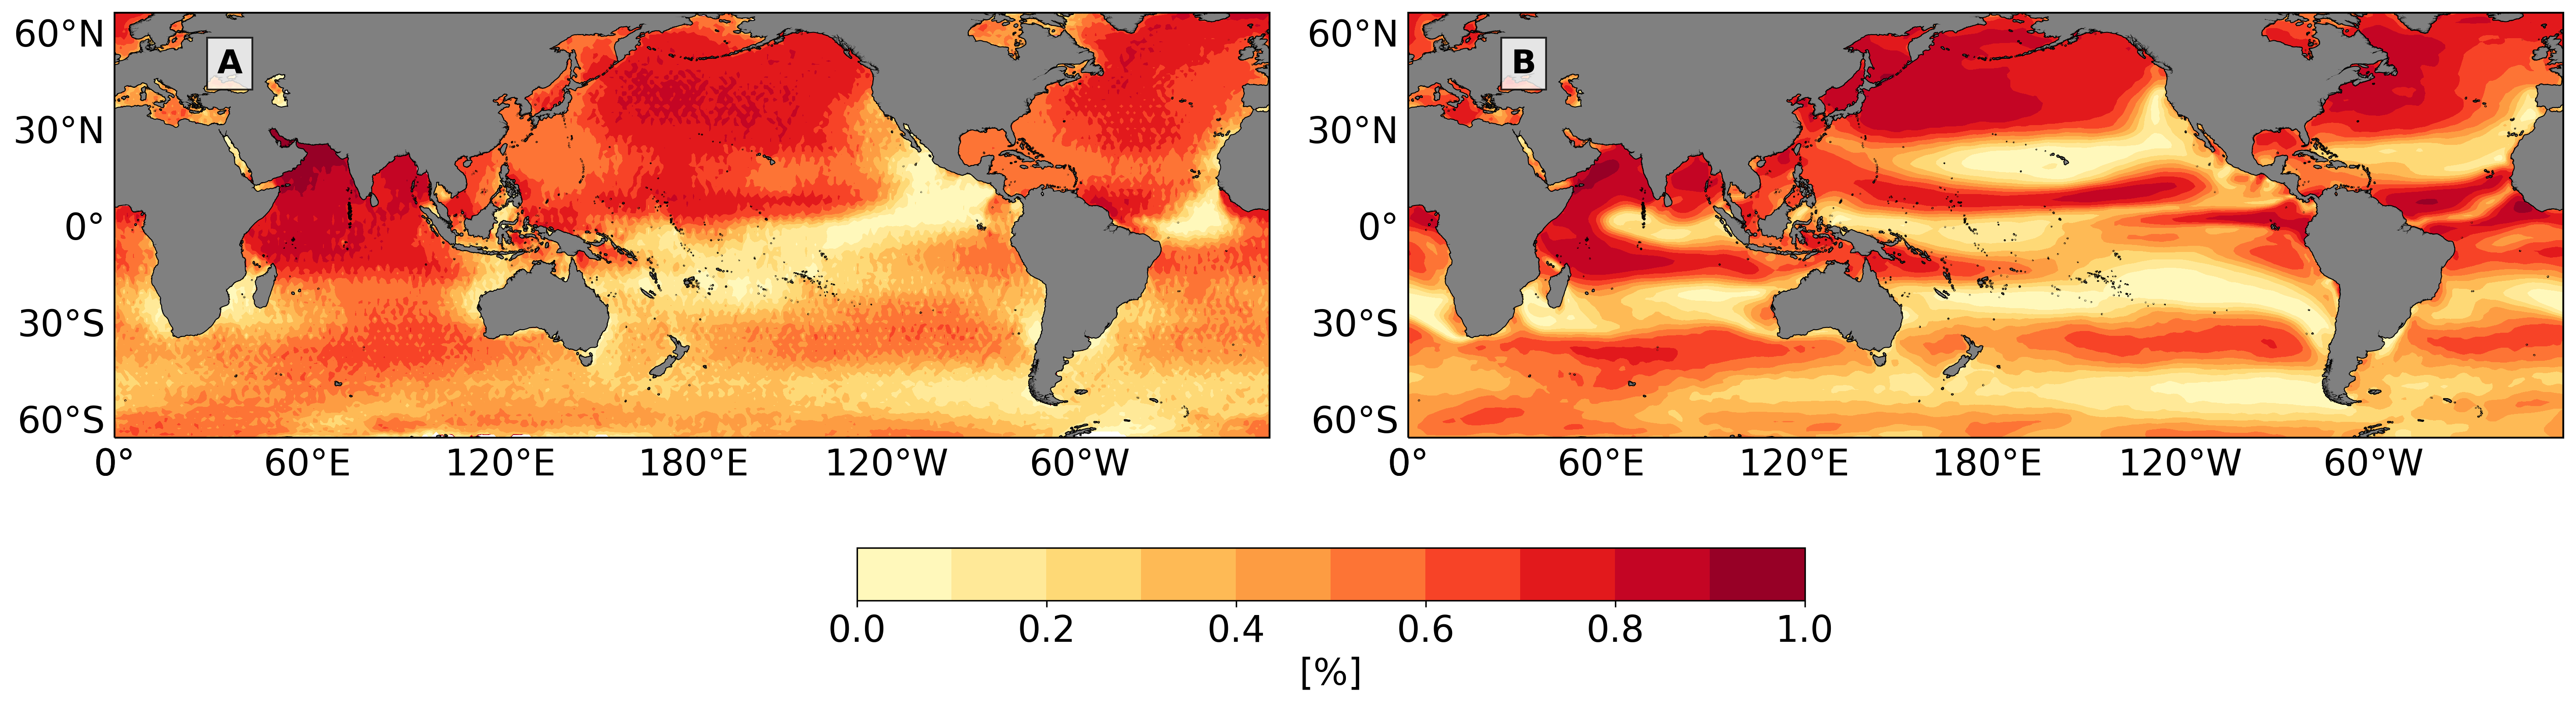
\includegraphics[width=1.0\textwidth]{figs/lsf_parameters/ccmp2_ifremer_goodness_of_fit_5_par.png}
\caption{Global map of Coefficient of determination for Ifremer SWH (A) and CCMP2 WSP (B) using Unweighted Annual and semi-annual Least Square Fit from January 1st, 1993 to December 31st, 2015 for a metric of the goodness of fit of the model.}
\label{Ifremer_ccmp2_lsf_gof}
\end{figure}

\subsection{Regional Climatologies of SWA Regions}

In order to obtain a closer look at the seasonal cycle within these SWA regions, climatologies or monthly mean SWH and WSP time series were computed from January 1st, 1993 to December 31st, 2015 within 4$^{\circ}$ by 4$^{\circ}$ grid boxes. Fig~\ref{reg_clima_nh} and Fig~\ref{reg_clima_sh} show the regional climatologies from SWA regions in the Northern and Southern Hemispheres respectively as well as the 4$^{\circ}$ by 4$^{\circ}$ regions within each SWA regions where the climatology is computed. From these climatologies, a clear difference is seen between Northern and Southern Hemisphere SWA regions. 

\begin{figure}[tbh]
\centering
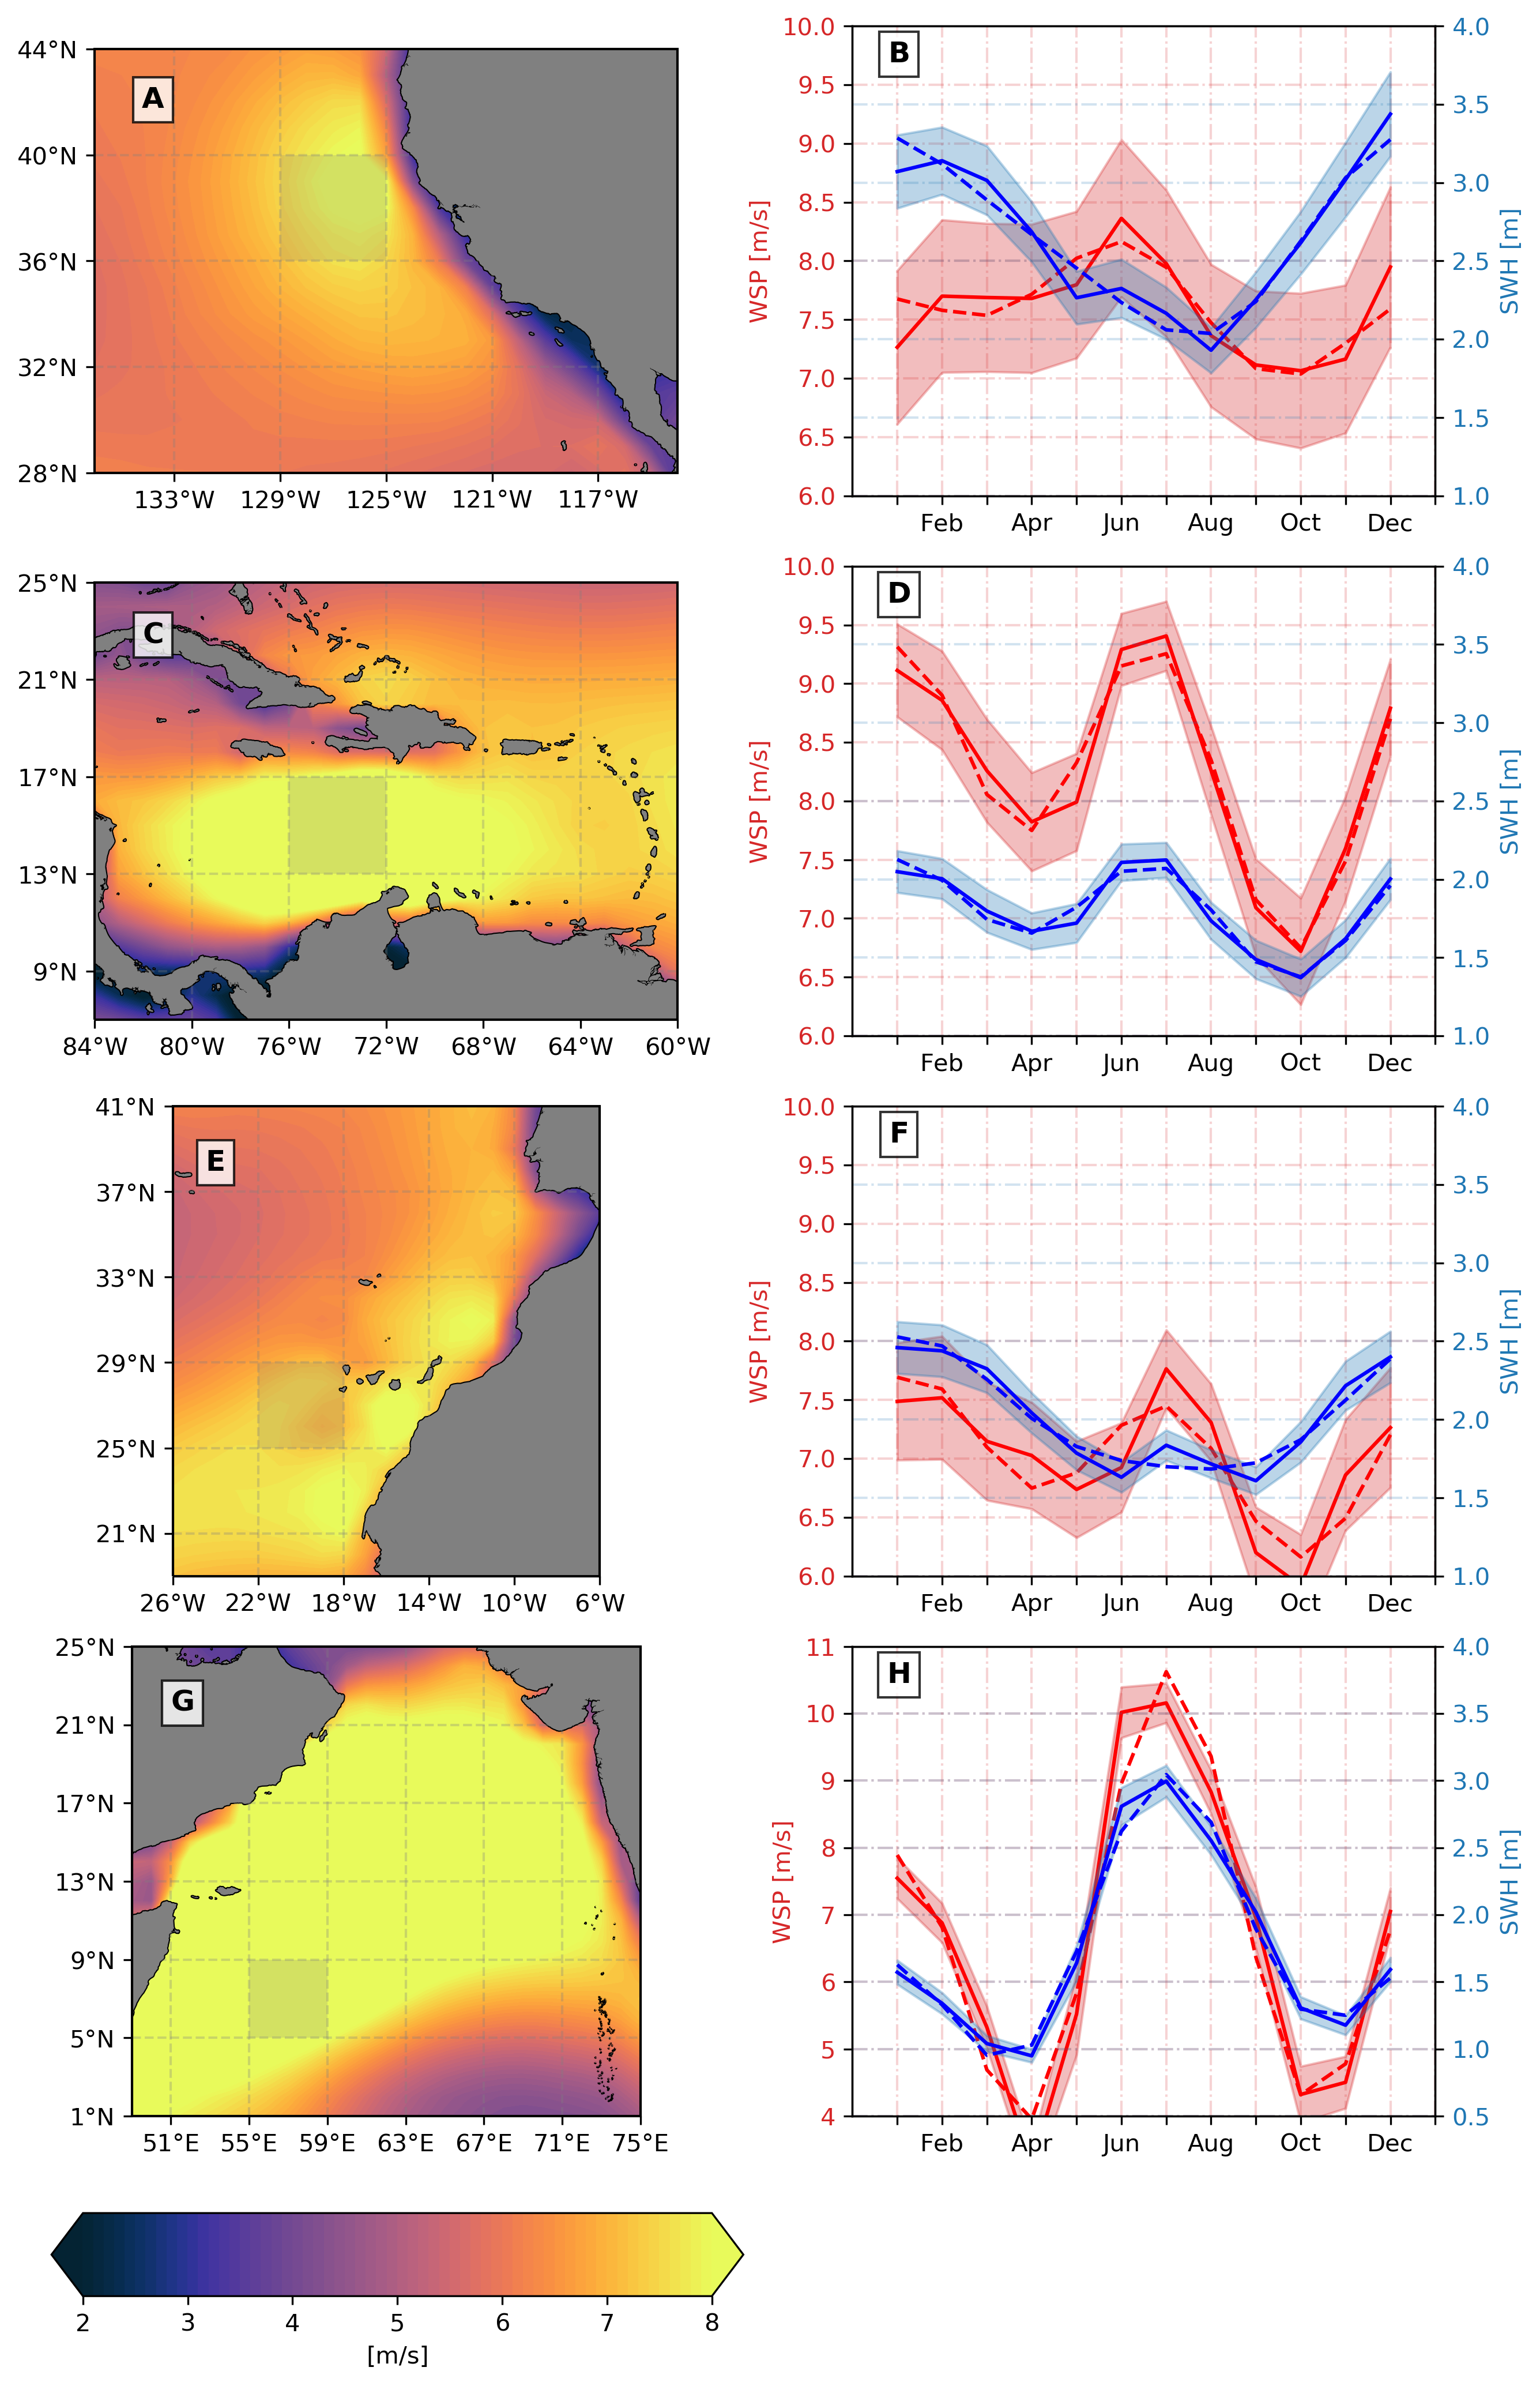
\includegraphics[width=0.5\textwidth]{figs/regional_climatologies/paper_regional_clima_nh.png}
\caption{SWA regional maps of WSP averaged over the months of June, July, and August (left column) with Ifremer SWH (solid blue curve) and CCMP2 WSP (solid red curve) climatologies in shaded 4$^{\circ}$ by 4$^{\circ}$ boxes within SWA regions located in the Northern Hemisphere. Shading in climatologies represents the standard error of the mean and dotted blue and red lines are the annual plus semi-annual cycle least-squares fitted to monthly climatology for SWH and WSP respectively. SWA regions include Northern California (A and B), Southern Caribbean Sea (C and D), North Africa near the coast of Morocco and western Sahara (E and F), North-Western Arabian Sea (G and H) }
\label{reg_clima_nh}
\end{figure}

\begin{figure}[tbh]
\centering
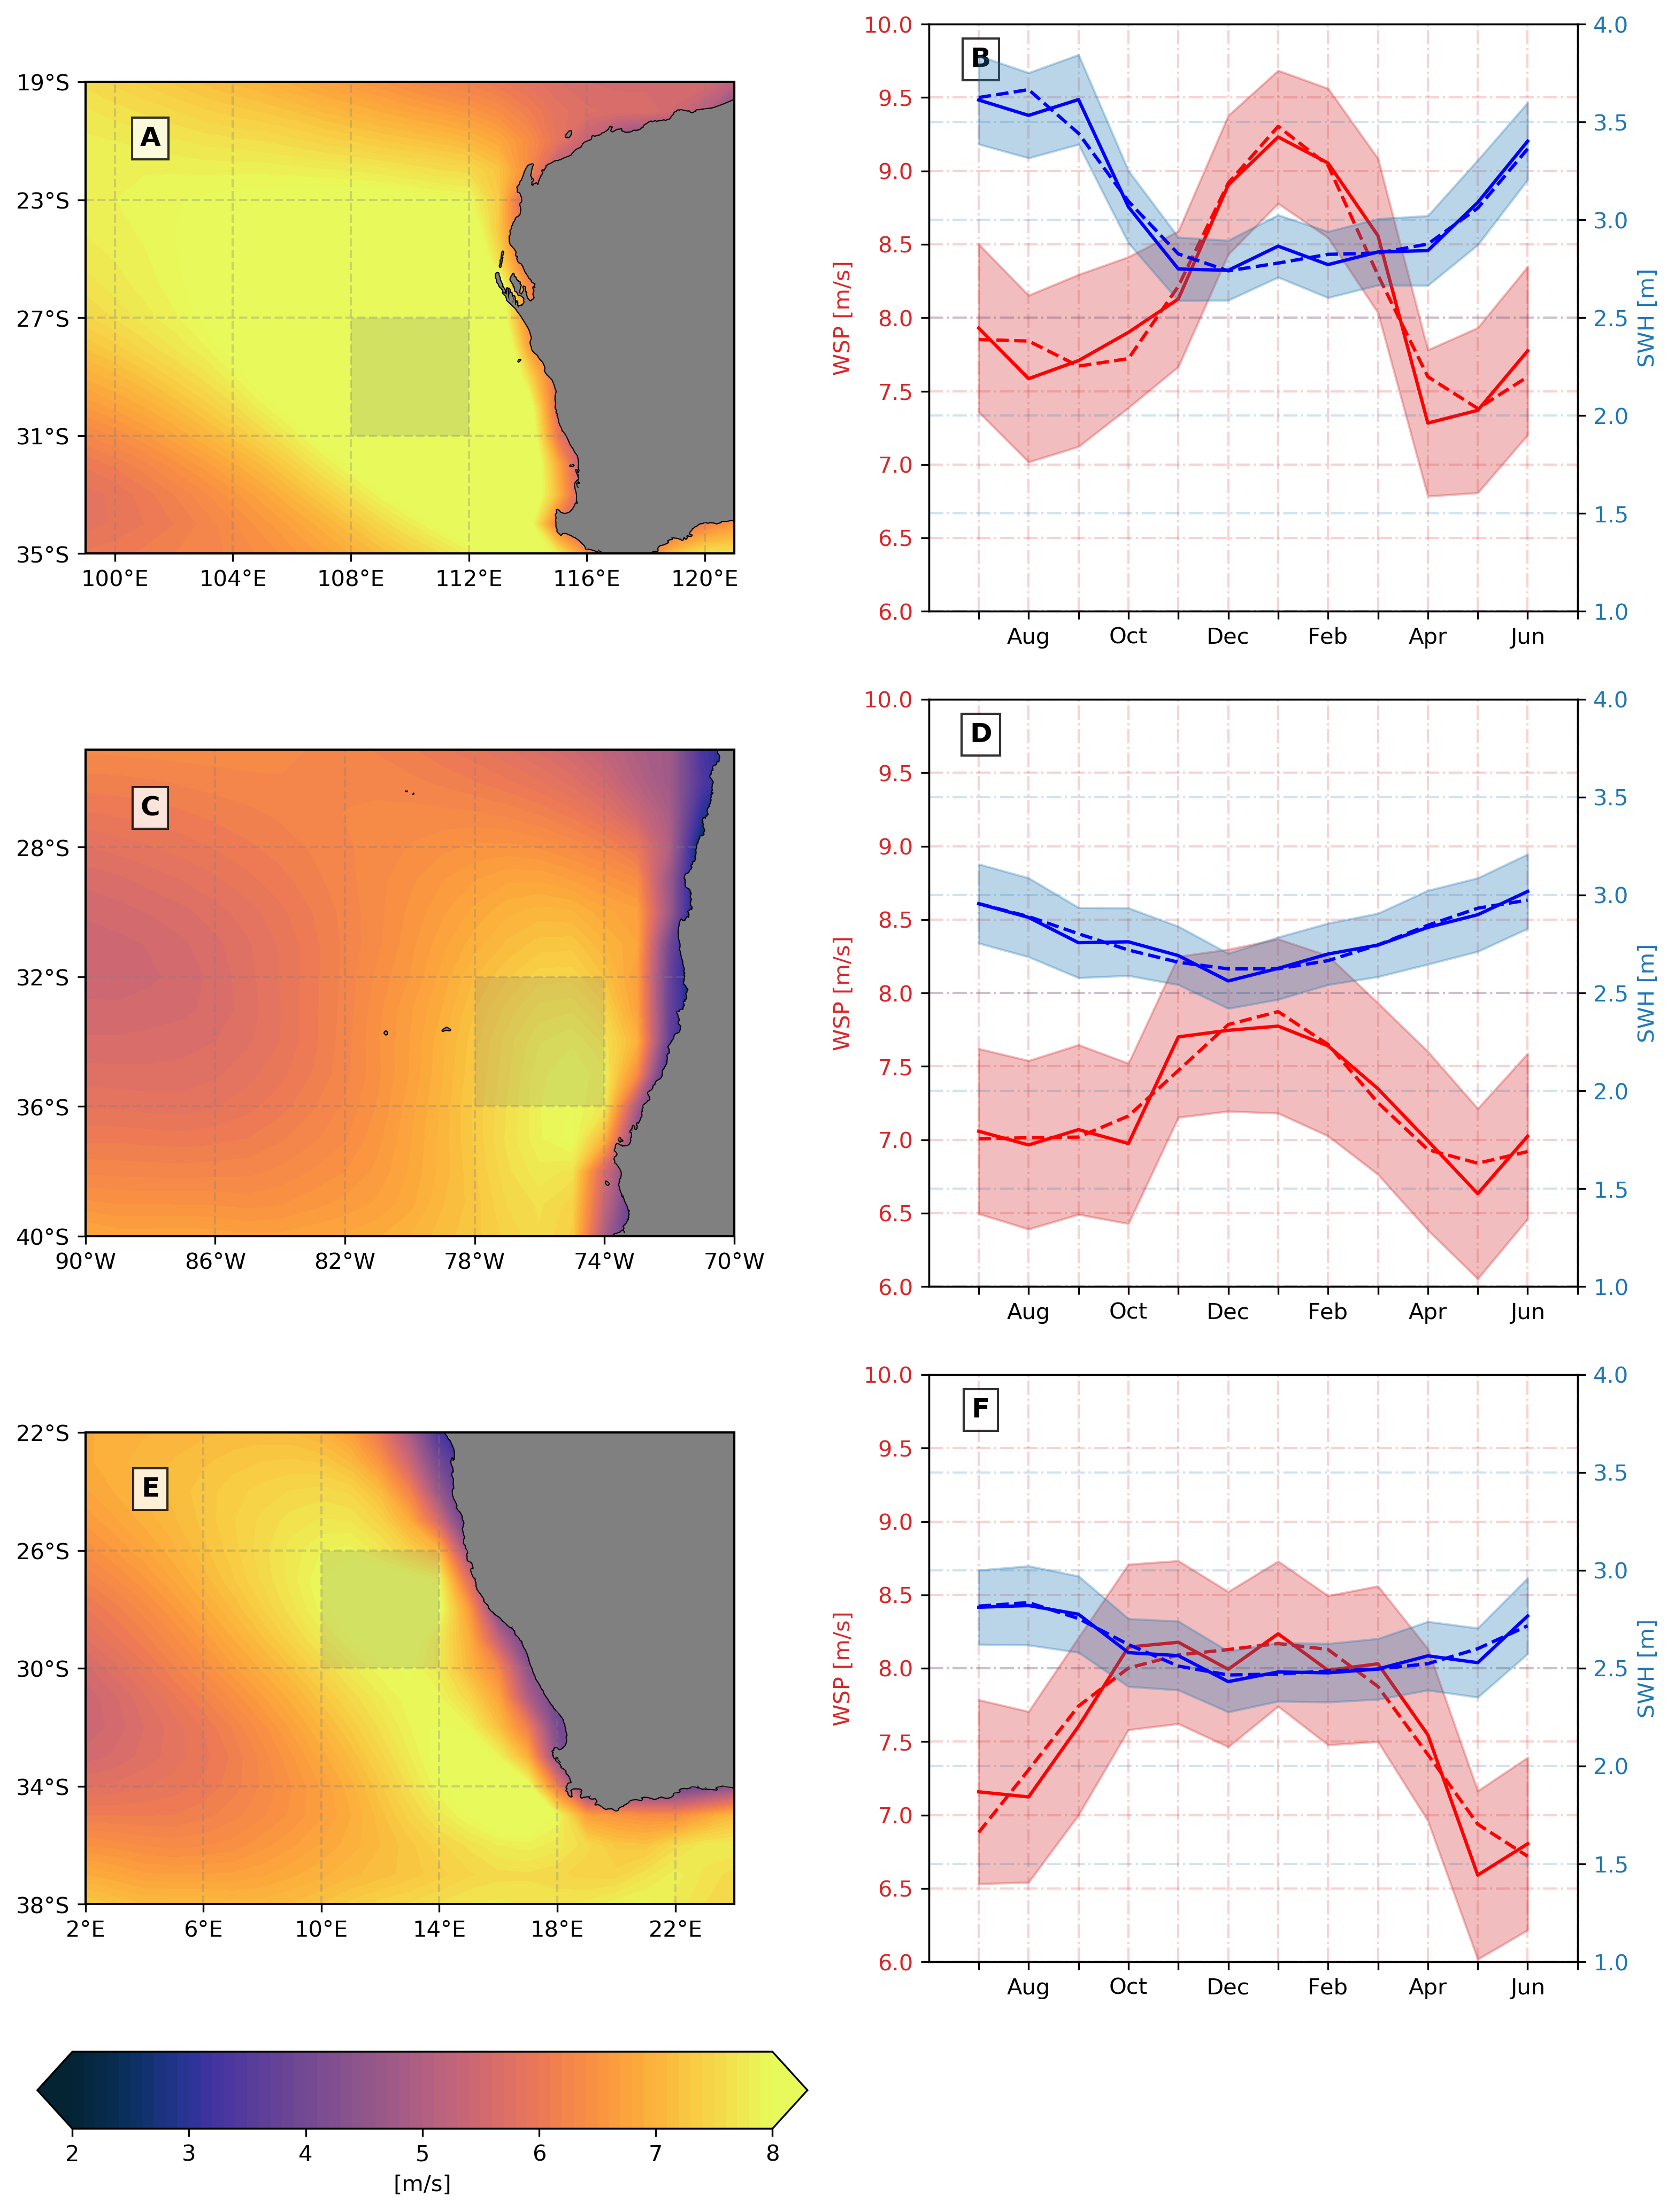
\includegraphics[width=0.5\textwidth]{figs/regional_climatologies/paper_regional_clima_sh.png}
\caption{SWA  regional maps of WSP averaged over the months of December, January, and February (left column) with Ifremer SWH (solid blue curve) and CCMP2 WSP (solid red curve) climatologies in shaded 4$^{\circ}$ by 4$^{\circ}$ boxes within SWA regions located in the Southern Hemisphere. Shading and dotted lines are as in Fig.~\ref{reg_clima_nh}. SWA regions include Western Australia (A and B), Central Western coast of South America near Chile (C and D), and South-Western Coast of Africa near Namibia (E and F)}
\label{reg_clima_sh}
\end{figure}


%In addition, by computing the residual at each time step between the same 5 parameter least square fit model used in the global analysis, it was observed that the residue values in SWA regions during the month of the local wind anomaly's presence had significantly larger than other residue values in the rest of the time series. However, this was not true for all SWA regions. Those SWA regions in monsoon regions with high magnitude deviations comparable to maximum of the seasonal cycle had lower residual values.

In all Northern Hemisphere SWA regions, the maximum in the WSP climatology occurs at the same time, when a deviation from the sinusoidal SWH seasonal cycle occurs. Examples include the Northern California and North African SWA regions (Fig~\ref{reg_clima_sh}B,F). Off the coast California, the WSP seasonal cycle reaches a maximum during the month of June. This peak is associated with an increase in SWH at the same time that the seasonal cycle is reaching a summer minimum. In the North African region off the coast of Morocco, a WSP maximum and a deviation from the SWH seasonal cycle are present in the month of July. In the Southern Hemisphere, the maximum in the WSP occurs during the austral summer in SWA regions, however there is only a small magnitude deviation from the SWH seasonal cycle occurring at the same time in the SWH climatology. Off the coast of western Australia (Fig~\ref{reg_clima_sh}B), a small magnitude deviation from the SWH annual cycle is present during the month of February when the maximum in the WSP climatology occurs. However, off the coast of Chile and Namibia (Fig~\ref{reg_clima_sh}D,F), deviations from the seasonal cycle are not present at all in the SWH climatology. Therefore, we propose that Southern Hemisphere SWA regions' (Fig~\ref{reg_clima_sh}) local wind forcing have comparatively less pronounced influence on the wave climate than in the Northern Hemisphere. This is presumed to occur because the magnitude of the deviation in the SWH cycle is determined by the local conditions and characteristics of the wave field within the region. Local conditions refers to the exposure and distance of the SWA region from remotely forced waves generation regions. In other words, how sheltered the SWA region is to regions with storms that produce high SWH remotely forced waves. By looking at looking at the two extreme cases of heavy sheltering and high exposure, the magnitude of the deviation from the SWH seasonal cycle can be explained. 

In the southern Caribbean Sea, the SWH climatology is in phase with the WSP climatology in Fig~\ref{reg_clima_nh}D. This implies that local wind events, including the wind anomaly during boreal summer and other wind events, predominately generate the waves within the region. This is due to the SWA region having little exposure to waves propagating from the high latitudes of the northern or southern Atlantic resulting in little of the wave energy being remotely forced. This sheltering from remotely forced waves is due to the Caribbean islands that ring the Caribbean sea (Fig~\ref{reg_clima_nh}C). The resulting seasonal variability, including the annual and semi-annual cycles, of this region is thus primarily set by local wind events within the Caribbean sea. Now by analyzing the increase in SWH occurring during the boreal summer due to the wind anomaly, the magnitude of this increase in SWH is relatively large such that the local maximum in SWH during the boreal summer is of similar or equal magnitude to the local maximum of the annual cycle. Therefore, the local wind anomaly significantly alters the climatology of SWH because the wave field tends to be dominated by locally forced wave for the majority of the year. This increase in SWH due to the wind anomaly also causing two maxima in SWH per year. This explains the near out of phase values seen in the Caribbean sea with respect to the rest of the Northern Hemisphere (Fig~\ref{Ifremer_ccmp2_lsf_chars}E). In addition, in Fig~\ref{Ifremer_ccmp2_lsf_chars}C,D, the large semi-annual cycle in the SWH and WSP semi-annual amplitude maps is clearly seen in the South Caribbean Sea due to the local wind anomaly. A similar semi-annual pattern occurs in the Arabian and South China seas, where monsoon winds generate high locally forced waves. The Arabian Sea has a similar wave climate to the South Caribbean with the wave field having a high tendency to be dominated by locally forced waves, however, this SWA region is not sheltered from remotely forced waves that propagate up from the Southern Ocean. This examples the high magnitude increase in the SWH climatology during boreal summer (Fig~\ref{reg_clima_nh}H). 

Off the coast of Western Australia, the increase in the SWH climatology during austral summer has small magnitude due to this SWA region having high exposure to the Southern Ocean where larger storms produce larger SWH remotely forced waves. These waves propagating into the SWA region cause there to be a high mean SWH which the SWH seasonal cycle oscillates about. These remotely forced waves of large amplitude overwhelm the wave field within the SWA region and cause the locally forced waves to have significantly less affect such that locally forced waves are less likely to dominate the wave field from the remotely forced waves. Therefore, the remotely forced waves overwhelm the locally forced waves and tend to dominate the wave field for a significant majority year with a slight exception during January in the austral summer. During January, the wave field tends to be dominated by locally forced waves and causes the slight increase in SWH. For the other two SWA regions in the Southern Hemisphere, the wave field is tends to be dominated by remotely forced waves all year round.  

We conclude that the magnitude of the deviation in the SWH cycle is determined by the local conditions and characteristics of the wave field within the region. Consequentially, the magnitude of the deviation from the SWH seasonal cycle is less than Northern Hemisphere SWA regions.    

From each of these climatology of SWA regions (Fig~\ref{reg_clima_sh}, Fig~\ref{reg_clima_nh}), it is also observed that significance of the deviation varies from region to region. The significance of deviation from the seasonal cycle can be determined by considering the standard error of the mean (Figs.~\ref{reg_clima_nh},\ref{reg_clima_sh}). In regions with high variance, the standard error of the mean is large enough that the deviation from the seasonal cycle is not statistically significant. This is seen in the west coast of Australia, coast of Chile, and the coast of Namibia.  

%possible look at the Chi-square value at time step such that we normalize the residue (model - data) by the standard error of the mean in order to determine statistical significance of deviation. By normalizing the residue with the standard error of the mean at each time step, a chi-square statistic can be obtained to determine which deviations from the seasonal cycle are statistically significant.

To comprehend the global extent of anomalous local surface winds over the world oceans and their possible influences on the local wave field, the fraction of the world's oceans experiencing anomalous winds was computed using WSP annual cycle phase calculated from CCMP2 daily data. WSP phase is categorized as anomalous when the WSP phase is greater than $-\frac{\pi}{2}$ in the Northern Hemisphere corresponding to the maximum in WSP annual cycle occurring outside of boreal winter months and greater than $\frac{\pi}{2}$ and less than 0 in the Southern Hemisphere corresponding to the maximum in the WSP annual cycle occurring outside of the Austral winter months. Observe that these wind anomalies are generated by a broad range of atmospheric forcings other than the expansion fan wind anomaly focused in this study. In order to compute this fraction, the world oceans where partitioned into southern and northern hemisphere basins including Indian Ocean, North and South Pacific, and North and South Atlantic Basins. Marginal Seas were mostly excluded as well as the equatorial regions across the Pacific and Atlantic oceans. We found that approximately 16.4\% of the world oceans have anomalous high WSP during the spring, summer and fall  months when it would be though to have lower WSP in the region. Fig~\ref{frac_wsp_anomaly} shows geographically where these wind anomalies occur. This calculation is approximate and not highly rigorous, however it gives a general impression of the larger extend and the geographic locations where these wind anomalies occur. All SWA regions are considered as anomalous except for the Arabian Sea. These regions categorized as having anomalous WSP phase may have a higher probability of the wave field being dominate by the local forced waves. However, this is depended on the local conditions of the wave field during the spring, summer, and fall months as discussed previously. 

 \begin{figure}[tbh]
\centering
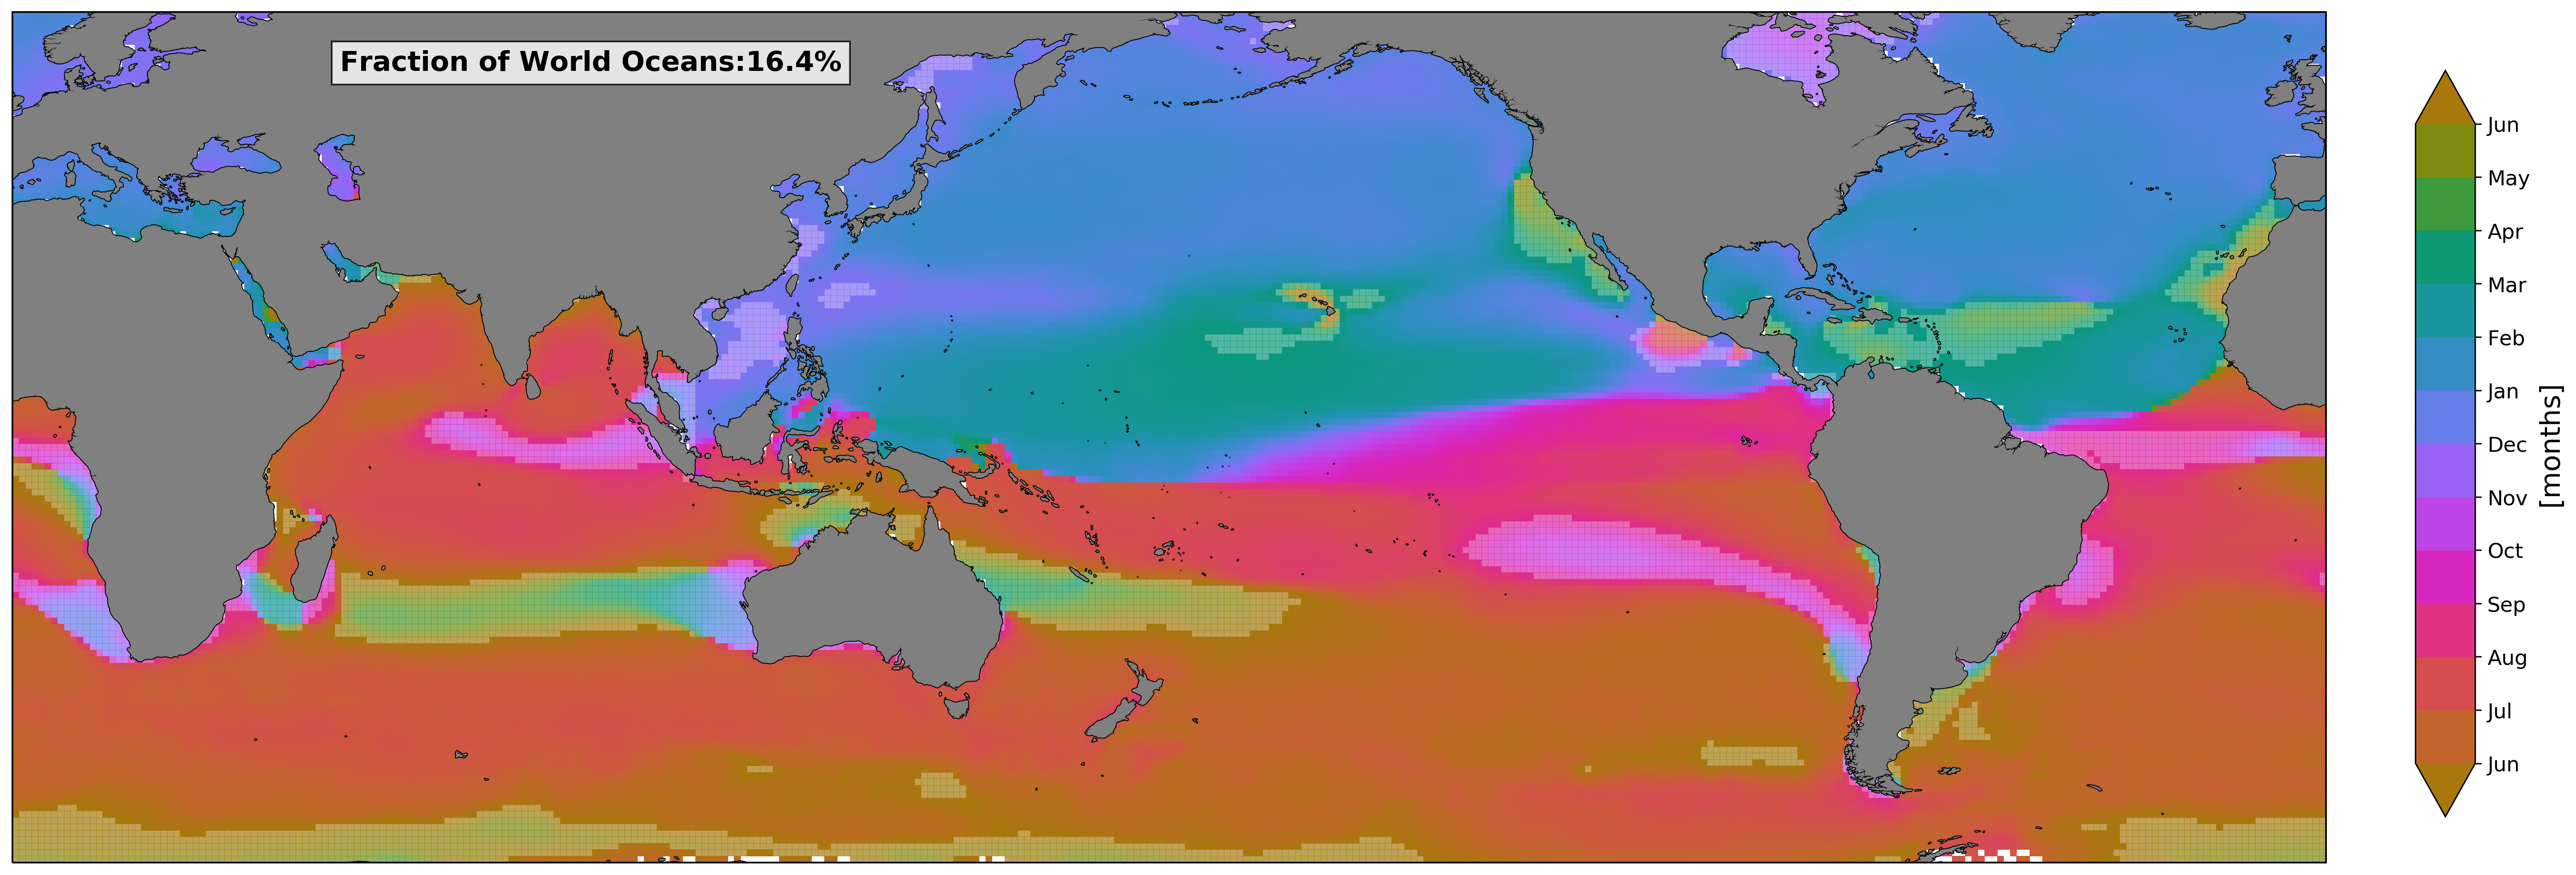
\includegraphics[width=0.5\textwidth]{figs/supplemental_figs/partitioned_ocean_anomaly.png}
\caption{WSP annual cycle phase with gridded and lighter regions indicating anomalous wind regions}
\label{frac_wsp_anomaly}
\end{figure}


\section{Wind-sea vs. Swell Dominance in SWA Regions}

\subsection{Local vs. Remotely Forced Waves}

In order to evaluate whether SWA region waves are generated by local wind events or remote storms, we use wave age information to classify waves as locally or remotely forced. During a storm, wind blows over a length of ocean surface called fetch at certain speed and for a given time duration, generating a packet of waves. Initially, waves that are formed by the wind are categorized as locally forced waves since the atmosphere is still supplying energy and momentum to the waves. These local forced waves are commonly called wind-seas. The frequency or wavenumber spectrum is evolving as wave height, frequency, and period of the waves grow. These waves tend to have shorter periods (or high frequency and wavenumber) and thus travel at slower phase speeds than long period waves. \citet{ardhuin2009observation} observed swells propagating across ocean basins using satellite altimetry data from ENVISAT and showed that steep swell waves lose a significant fraction of there energy (up to 68\%) over distances of 2800 km due to the laminar to turbulent transition in the air-side boundary layer. Wind-sea waves tend to be steep because of their short periods and high amplitudes, and this leads to significant dissipation over relatively short distances \cite{ardhuin2009observation}. In addition, wind-sea wave dissipation could also be due to small scale wave-wave interactions, wave-current interactions and other atmospheric forcing. Therefore, the wind event must be relatively in close proximity to wind-sea waves. Once the wind is no longer inputting energy and momentum into the waves, the waves are categorized as remotely forced waves. Remotely forced waves are commonly called fully developed seas or swell. In the case of swell waves, the wave field's frequency or wavenumber spectrum is set and is no longer evolving. These waves tend to have long periods (or low wave frequency and wavenumber) and have the ability to traverse long distances at higher phase speeds than short period waves \cite{snodgrass1966propagation}. This leads to the dispersive nature of deep water surface gravity waves \cite{snodgrass1966propagation}.   

Waves measured by satellite altimeters represent a superposition of local wind waves and remotely generated swell, and the altimeter does not distinguish frequency, period, or direction. This is due to shape of the backscatter radiation off the sea surface received by the satellite altimeter obtaining an average of the variability of the wave height present in the satellites footprint \cite{chelton2001satellite}. Therefore, the SWH obtained from satellite altimetry represents the wave height of the dominate waves within the wave field where these waves may be generated locally or remotely. Globally, the wave field is consistently dominated by swell \cite{chen2002global,semedo2011global}.

%However, the dominant wave height within the satellite's footprint is only recorded. Therefore, local wind events have varying degrees of influence on the annual cycle of swh depending on the amount of remotely forced waves that enter a given region. 

To distinguish between wind-sea and swell waves, wave age may be used. Wave age quantifies the stage of development of waves and is therefore used to separate locally forced waves from remotely forced waves through an empirically and theoretically determined criterion \cite{alves2003revisiting}. The wave age criterion is defined as 
\begin{equation}
     \mbox{\rm Wave Age} = \frac{C_{p}}{U_{10}},
 \end{equation}
where $C_{p}$ is phase speed of the surface gravity wave or the speed of an individual wave crest and $U_{10}$ is the wind speed 10 meters above the ocean surface. The separation value used in our analysis to distinguish locally and remotely forced waves is 
\begin{eqnarray}
     \frac{C_{p}}{U_{10}} & > & 1.2\quad {\mbox{\rm Remotely Forced Waves}} \\
     \frac{C_{p}}{U_{10}} & \leq & 1.2\quad {\mbox{\rm Locally Forced Waves}}
\end{eqnarray}
This criterion has been chosen and has empirically shown that wave growth stops or at least becomes very slow when wave age is greater than 1.2 \cite{donelan1992growth}. This corresponds with waves crests travelling 20\% faster than the wind speed 10 meters above the ocean surface, so that the waves are outrunning the wind and not able to receive further wind energy input. We assume that the satellite observes deep water waves, with a wavelength much less than the water depth. For deep water waves, the deep water dispersion relationship yields a peak phase speed: 
\begin{equation}
    C_{p} = \frac{g}{2\pi f_{p}}
\end{equation}

%In addition, using the directional spectrum, \citet{echevarria2019seasonal} was able to categorize the wave field into five main wave modes for the first empirical orthogonal function in their principal component analysis. This illustrated that the first mode EOF explains variability in the high latitudes while multiple modes are needed in the equatorial region. Each of these modes have been associated with different wind systems that generate these wind waves. In all multi-modal regions, all these modes overlap and coexist with each other in order to give us the seasonal variability of the wave climate \cite{echevarria2019seasonal}.

\subsection{Probability of Swell: Wave Age Method}

Using wave age or other wind-sea and swell separation techniques, probability of swell can be obtained to illustrated the amount of times the wave field is swell-dominated for a given grid point as a fraction of the total amount of wave events which includes wind-sea dominated and swell dominated events:
\begin{equation}
    \mbox{\rm Probability of swell} = \frac{N_{swell}}{N_{total}}
\end{equation}
where $N_{swell}$ is the number of time steps with wave age exceeding 1.2 representing a swell dominated wave field and $N_{total}$ is the total number of observations in the time series .

Probability of Swell has been computed globally before by \citet{jiang2013global} and \citet{semedo2011global}. \citet{jiang2013global} used collocated satellite altimetry SWH and radiometer WSP from the Jason-1 satellite mission to compute the probability of swell using a wind-wave relationship derived from the Wave Modeling (WAM) Program which was able to separate wind-seas from swell. Global seasonal maps of probability of swell showed that the SWH observations by satellite altimetry are categorized primarily as remotely forced waves in all oceans with lower probability of swell in the Southern Ocean, in coastal regions, and along common storms tracks \cite{jiang2013global}. The probability of swell also undergoes a seasonal cycle with a decreasing seasonal cycle amplitude when approaching the equator. This decrease in probability of swell indicates an increase in the amount of wind events generating wind seas that dominate the wave field. \citet{semedo2011global} computed probability of swell using wave age as the separation criterion with European Centre for Medium-Range Weather Forecasts Re-Analysis (ERA-40) wave reanalysis. \citet{semedo2011global} found high probability of swell consistently throughout the world oceans implying that swell dominates the wave field \cite{semedo2011global}. Building on this analysis, wave energy spectra from ERA-40 was used separated into wind-sea and swell components using WAM separation frequencies and then SWH, mean wave period (MWP) and mean wave direction (MWD) were computed for each components. From seasonal maps of SWH decomposed into swell and wind sea components, the swell SWH was found to be always higher than the wind-sea component implying that swell dominates the wave spectra \cite{semedo2011global}. 

By computing probability of swell globally for each season using wave age, probability of swell in SWA regions can confirm if the wave field observed during the spring months in SWA regions were dominated by wind-seas generated by the local wind anomaly or dominated by swell propagating from distant storms.  

To calculate phase speed of waves and therefore wave age, we used Wave Watch 3 (WW3) modeled data with peak frequency. The Climate Forecast System Reanalysis (CFSR) winds provided the forcing to WW3 wave model in order to obtain the bulk parameters SWH and peak frequency with 6 hourly temporal and 0.5 degree spatial resolution. Wave age was computed after decreasing the spatial resolution of WW3 peak frequency and CFSR WSP to 1 degree and the temporal resolution to daily time steps. The WW3 and CFSR products were used instead of the coupled ECMWF wind product and WW3 wave parameters because CFSR WSP forcing WW3 SWH has more seasonal variability, and prediction accuracy improves in recent years \cite{stopa2014intercomparison}. However, the WW3 and CFSR data sets has some potential biases, including overestimation of SWH and WSP as compared to in situ buoy observations and less temporal homogeneity than ECMWF forcing WW3 model which manifests itself as a slightly less smooth time series allowing CFSR and WW3 to more accurately model extreme weather events \cite{stopa2014intercomparison}.  

%In order to validate that the modelled WW3 CFSR data agrees with observation made by the Ifremer satellite altimetry SWH product and CCMP version 2 WSP product, the WW3 SWH and WSP climatologies are computed and overlaid on the Ifremer SWH and CCMP2 WSP climatology maps. In addition, global maps of swh and wsp parameters of the 5 parameter least square fit are computed. Visually, it is observed that there is relatively good agreement with the the seasonal cycle monthly mean values between WW3 and Ifremer and CCMP2 data. Notice that there comparisons are performed after significant temporal and spatial averaging. Therefore, this is not a statement for the actual point by point agreement of modelled data versus active remote sensing measurements. Averaging has reduced some of the variability and uncertainty within the two data set which has allowed for the comparison to be viable.

Before computing wave age with WW3 peak frequency using CFSR winds, we preformed an elementary comparison test between remotely sensed SWH and WSP observations and WW3 SWH and CFSR WSP to understand how well the WW3 SWH and CFSR WSP were representing the observational data. This validation process included computing regional climatologies of WW3 SWH and CFSR WSP data in the same regions which that observational SWH and WSP climatologies were computed. In addition, the least-squares fit annual and semi-annual model was fitted to WW3 SWH and CFSR WSP and parameters of model were computed. Before preforming comparison, the WW3 and CFSR data resolutions were decreased spatially to 1$^{\circ}$ by 1$^{\circ}$ and temporally to monthly time steps in order to match the data resolution of the least squares fit and regional climatology analysis. This prevents the model's small-scale spatial variability from artificially reducing correlations between the modelled and observed data. Regional climatologies of WW3 SWH and CFSR WSP data are compared to the Ifremer SWH and CCMP2 WSP in Fig~\ref{ww3_ifremer_ccmp2_compare}, and the parameters  of the least-squares fit of WW3 SWH and WSP (not shown). Both regional climatologies and parameters of the 5 parameter least square fit show high agreement in all of the SWA regions. This means that the amplitude and phase of the annual and semi-annual cycles agree well in SWA regions. However, there are small disparities present. For the regional climatologies, the model underestimates or agrees well with SWH in all SWA region climatologies except off the California coast where the model consistently overestimates (Fig~\ref{NH_model_comparison}). The model overestimates WSP off the coasts of California, Chile, and Namibia (Fig~\ref{NH_model_comparison},Fig~\ref{SH_model_comparison}). In SWA regions off the coast of west Australia, north Africa, south Caribbean, and the Arabian Sea, the model overestimates the climatological maxima while underestimating the minima. 

What are the consequences of overestimating or underestimating WSP on the probability of swell if assuming peak frequency is unbiased and is held constant? By overestimating WSP, wave age would decrease (increasing the denominator and decreases wave-age ratio) making it more likely for wave age drop below 1.2 and the wave field to be categorized as wind-sea dominated. This would lead to an decrease the probability of swell. Therefore, there may be a bias toward low probability of swell in SWA regions including Northern California, Chile, and Namibia. Using the same rational as before, for the southern Caribbean and Arabian Seas, there is a bias toward lower probability of swell during the boreal summer when the local wind anomaly occurs due to CFSR overestimates WSP. For northern Africa, the probability of swell would have very little bias introduced by the WSP data due to the high accuracy of the model. For Western Australia, there is a slight bias toward lower probability of swell in the austral summer and higher probability of swell in the austral winter due to the CFSR underestimating WSP. Next, peak frequency must be validated by comparing it with in situ observations. Performance assessments of WW3 peak frequency have been studied in the Pacific basin by \citet{hanson2009pacific} using the Wave Model Evaluation and Diagnostics System (WaveMEDS) to quantify the biases and overall performance scores for peak period for the entire wave field and for each component (wind-seas and swell) for the year 2000. The WW3 wave model had wind forcing from the high-quality, consistent, neutral stability wind fields NRAQ+ generated by the marine meteorology group at Oceanweather Inc. \cite{hanson2009pacific}. This is not the same wind forcing used to force the WW3 peak frequency data in this study, however, \citet{hanson2009pacific} has validated the peak frequency with realistic and reliable wind forcing. The WW3 modeled wave spectra is compared with wave spectra from seven deep-water buoy sites from the National Data Buoy Center (NDBC) and the Coastal Data Information Program (CDIP). \citet{hanson2009pacific} concluded that wave period agrees with in situ observations with a combined wind-sea and swell waves performance score of 0.93 for temporal correlations and 0.96 for quantile-quantile \cite{hanson2009pacific}. 

%There is very low differences of 0.01 in performance scores between wave components. The performance score ranges from 0 to 1, with 1 being an exact match between observations and hindcast modeled data. Having a higher quantile-quantile score than temporal correlations indicates that WW3 is better at modeling event distributions than correctly matching event times \cite{hanson2009pacific}. This means that a lag could exist in the time series between the onset of the wind event and the peak characteristics of the wave field. 

The validation of the wave parameter peak frequency occurs with buoys located primarily in the Northern Hemisphere pacific. Other ocean basins have still yet to be rigorously validated for peak frequency. With the fore knowledge that the performance of peak frequency is unknown in other ocean basins, we use peak frequency based on the high accuracy of the model in representing in situ observations in the pacific. 

%Assuming that Pacific assessment is a relatively good approximation for the assessment of other ocean basins, we can conclude that the peak period and therefore, the peak frequency is highly reliable with a significantly lower bias than the WSP bias. 

\begin{figure}[tbh]
\centering
\begin{minipage}{.5\textwidth}
  \centering
  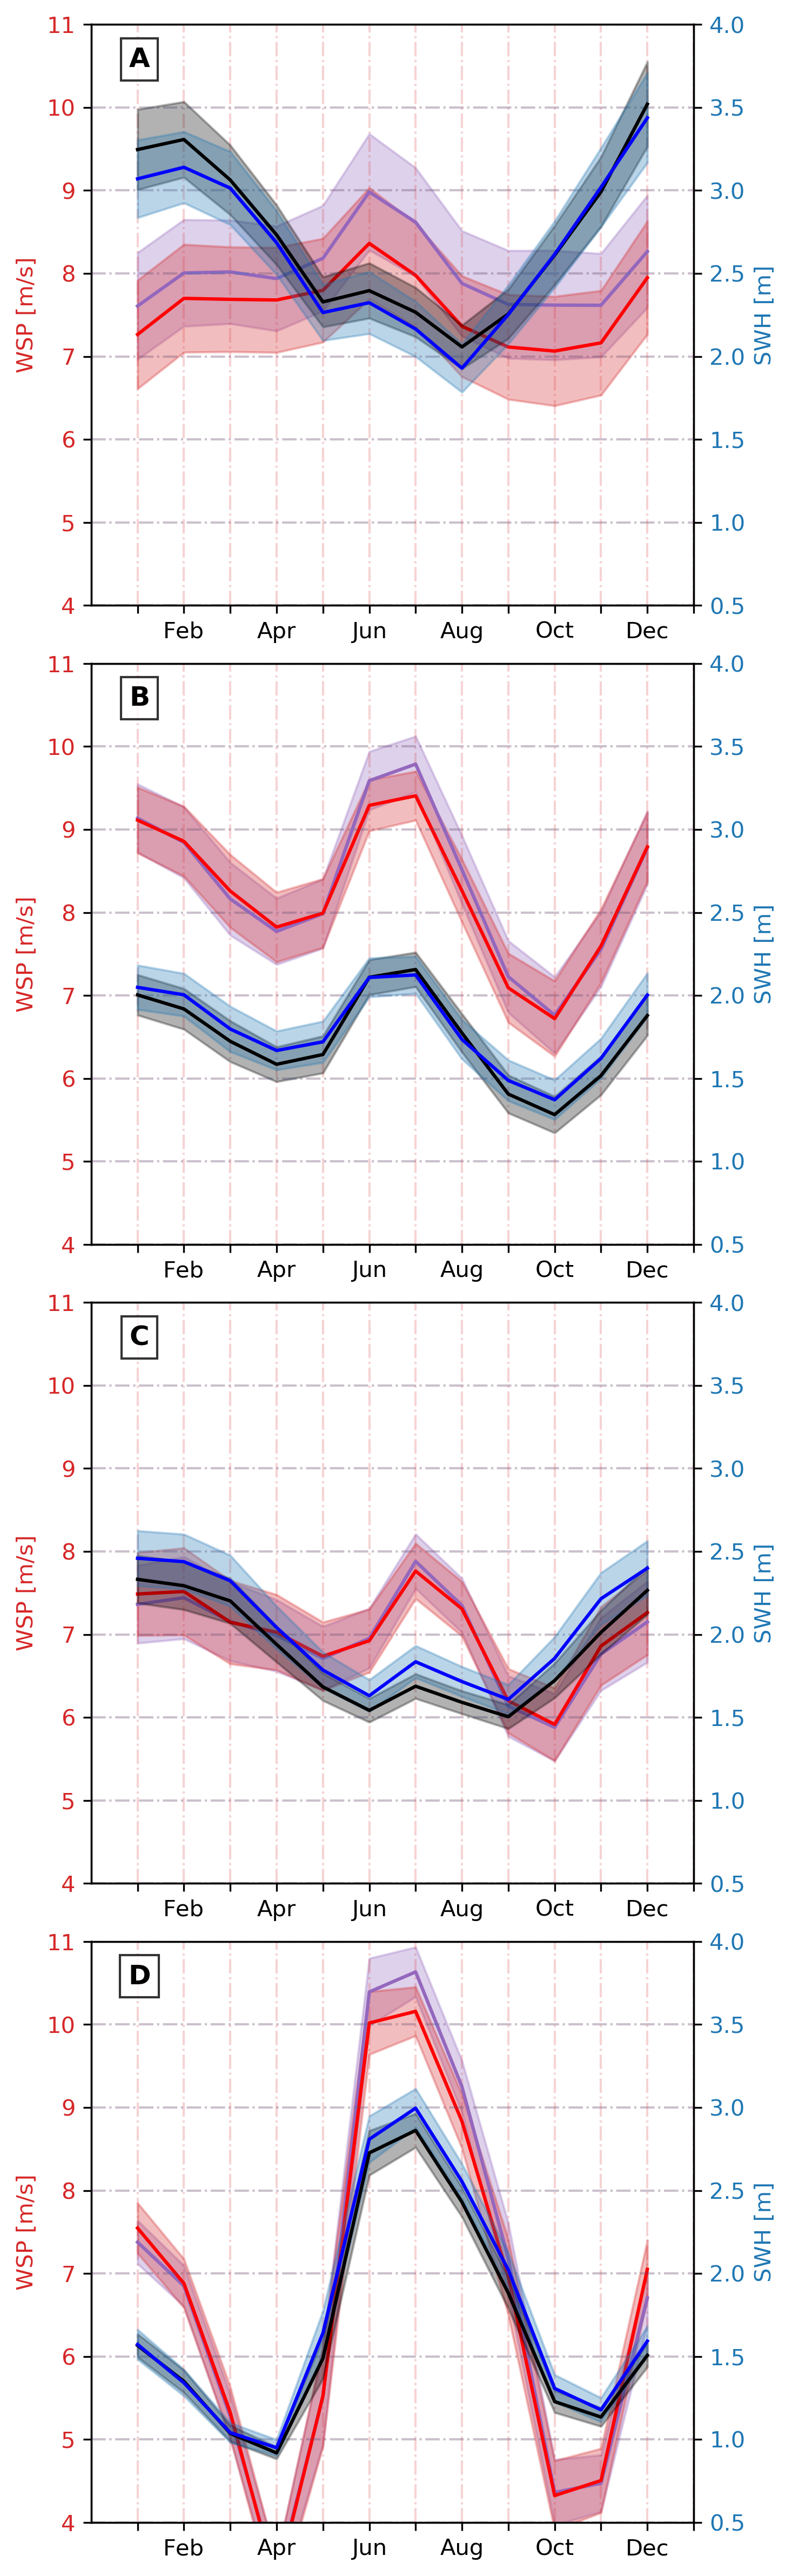
\includegraphics[width=0.5\textwidth]{figs/regional_climatologies/SWARs_reg_clima_4x4_nh_ww3.png}
  \caption{Northern Hemisphere SWA regions where (A) North California, (B) Southern Caribbean, (C) North Africa, and (D) Arabian Sea which are the same regions as in Fig~\ref{reg_clima_nh}}
  \label{NH_model_comparison}
\end{minipage}%
\begin{minipage}{.5\textwidth}
  \centering
  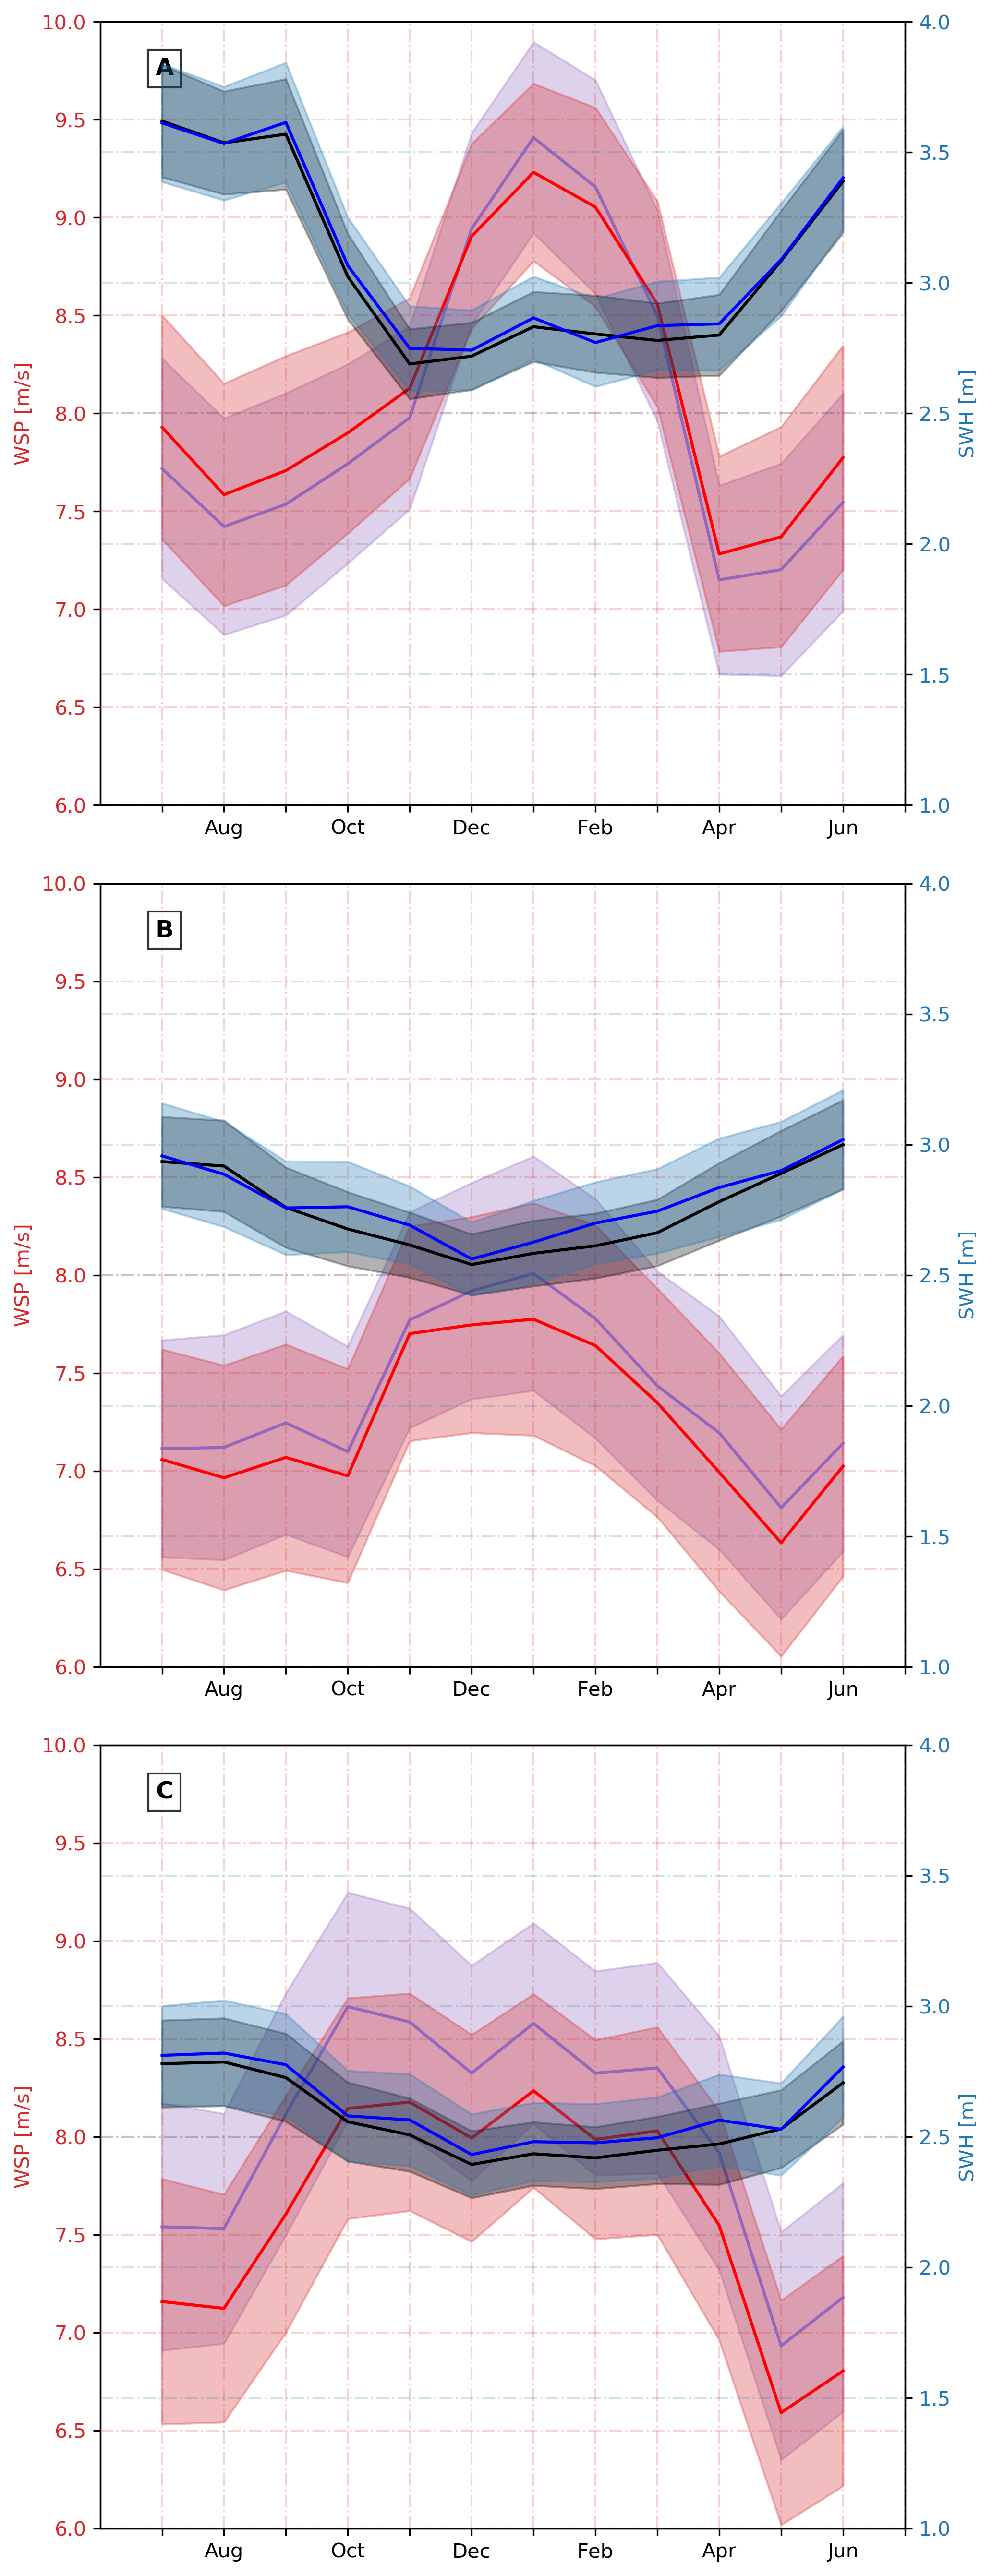
\includegraphics[width=0.5\textwidth]{figs/regional_climatologies/SWARs_reg_clima_4x4_sh_ww3.png}
  \caption{Southern Hemisphere SWA regions where (A) West Australia, (B) coast of Chile, and (C) coast of Namibia which are the same regions as in Fig~\ref{reg_clima_sh}}
  \label{SH_model_comparison}
\end{minipage}
%\caption{WW3 SWH and WSP climatology comparison with Ifremer SWH and CCMP2 WSP}
\label{ww3_ifremer_ccmp2_compare}
\end{figure}

%In order to determine the degree of remotely forced versus locally forced waves in SWA regions, we used the probability of swell ratio implemented by \citet{semedo2011global}:
%\begin{equation}
%    \mbox{\rm Probability of swell} = \frac{N_{swell}}{N_{total}}
%\end{equation}
%where $N_{swell}$ is the number of time steps with wave age exceeding 1.2 and $N_{total}$ is the total number of observations in the time series. $N_{total}$ is the sum of $N_{swell}$ and $N_{wind}$ where $N_{wind}$ is the number of time steps in the time series with wave age less than or equal to 1.2.

Figure~\ref{prob_swell_ww3} is a seasonal progression global map of probability of swell which agrees very well with \citet{semedo2011global} global maps of probability of swell for DJF and JJA. As observed in Figure~\ref{prob_swell_ww3}, SWA regions contained waves that were categorized as locally forced during the late spring and early summer months. This is illustrated by the probability of swell being significantly lower in SWA regions than the surrounding areas around SWA regions during the season when the wind anomaly occurs. For the northern hemisphere, off the coast of California, the probability of swell significantly drops to 90\% in the spring months and then below 75\% in the summer months. Similarly, off the coast of North Africa, probability of swell drops to between 90\% to 80\% in the spring months and then below 75\% in the summer months. Both the Caribbean and Arabian Seas are consistently below 75\% through the entire year. This means that the wave field is more frequently dominated by locally forced waves than remotely forced waves. Therefore, this result agrees with the hypothesis that the deviation from the SWH annual cycle is a result from locally forced waves dominating the wave field and causing a increase in SWH. For the Southern Hemisphere, the probability of swell in the SWA regions of West Australia, Chile, and Namibia is not as low as in other SWA regions. This would also agree with the hypothesis that the SWA regions in the Southern Hemisphere have wave fields that are dominated predominately by remotely forced waves (and dominated by locally forced wave on fewer occurrences) due to their proximity to the Southern Ocean leading to a less pronounced or nonexistent deviation from the SWH annual cycle. 

\begin{figure}[tbh]
\centering
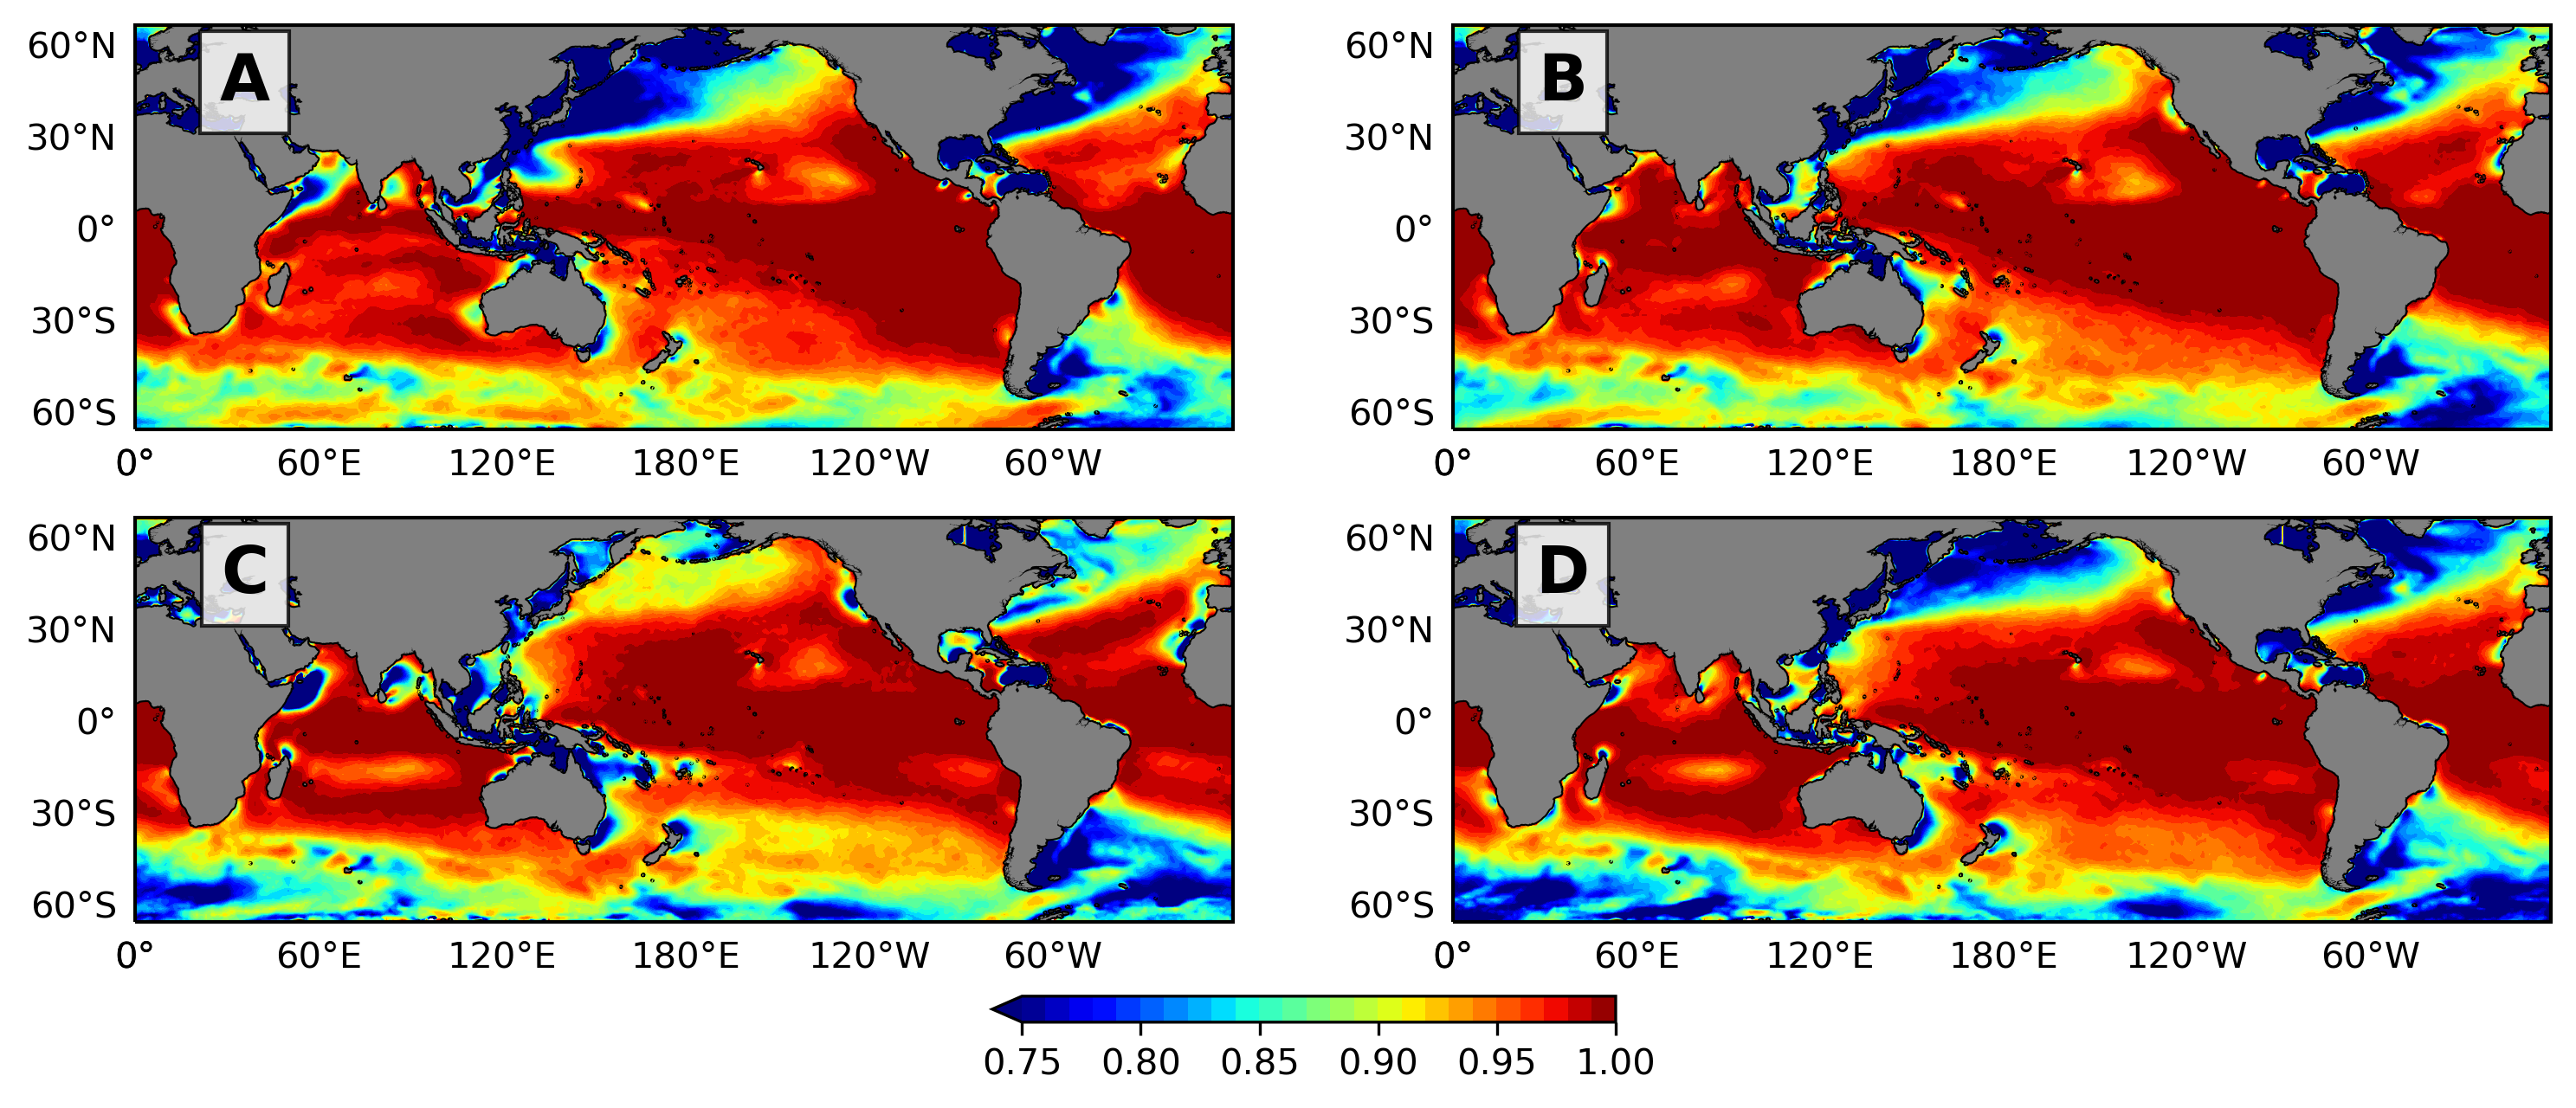
\includegraphics[width=1.0\textwidth]{figs/probability_of_swell/WW3_CFSR_prob_swell_seasons_2x2.png}
\caption{Seasonal progression of probability of swell using wave age criterion and WW3 peak frequency and WSP from January 1st, 1993 to December 31st, 2015 where (A) DJF, (B) MAM, (C) JJA, and (D) SON}.
\label{prob_swell_ww3}
\end{figure}

\section{Conclusion}

This study has analyzed the seasonal cycles of SWH and WSP by least-squares fitting annual and semi-annual cycles to satellite observations. In most of the ocean SWH is higher in winter, indicating a response to high-latitude winter storms that generate equatorward-propagating swell. Exceptions occur in a few eastern boundary current regions and other wind anomaly regions, where strong local winds in spring or summer generate wind waves that are out of phase with the winter storms. In the equatorial region, the boundary where the domains of dominance of Northern and Southern Hemisphere storm patterns setting the SWH annual cycle occurs off the equator in the Southern Hemisphere following the line where the amplitude of the SWH annual cycle vanishes. This boundary is hypothesized to be influenced significantly by Polynesian islands affecting the way waves propagate through this region. Using regional climatology analysis in 4$^{\circ}$ by 4$^{\circ}$ boxes, we find that in SWA regions, the SWH can deviate from a sinusoidal annual cycle with winter maximum, instead indicating direct response to local winds. In SWA regions, the fraction of wave variability attributed to local wind events varies depending on local conditions. 16.4\% of the world oceans including all but one of the SWA regions experience an anomalous WSP seasonal variability with the maximum of the WSP seasonal cycle occurring outside of the winter months of the respective hemisphere. The waves within each SWA region have low probability of swell during the spring and summer months of each hemisphere respectively. This implies that there is an increase in the number of times the wave field is dominated by wind-seas, supporting the hypothesis that the deviation from the SWH annual cycle results from wave that are locally forced by a local wind events.

Further research would include using spectral data from WW3 waves model forced by CFSR winds in order to separate wind-sea and swell parameters in SWA regions via spectral partitioning \cite{portilla2009spectral} to further validate the claim that the deviation in the SWH seasonal cycle occurs from local wind events. In addition, local wind events should be further investigated to evaluate whether local winds result from the same atmospheric coastal topographic processes as in California. 

By improving our understanding of the SWH climate globally with respect to the effects of local wind events, wave models can more accurately model and anticipate increases in SWH. Through understanding the wave climate in these SWA regions, we gain greater insight into determining at what times during the year remotely and locally forced wind waves dominate the wave field. Wave field's dominated by locally forced waves have strong interactions between waves and the lowest atmospheric layer \cite{cavaleri2012wind} due to the tendency of waves have short frequencies and steep. Processes involved in air-sea interactions that are amplifies by locally forced waves includes wave breaking and white capping. Both of these processes leads increase heat and mass fluxes from ejecting sea spray including aerosols into the atmospheric boundary layer, injecting bubbles into the ocean, and causing waving-induced mixing in the upper ocean layer \cite{cavaleri2012wind}. Sea-state dependent surface wave modulated fluxes of momentum, energy, heat and mass are all essential for climate models being able to close budgets to full describe the coupled ocean-atmosphere system \cite{cavaleri2012wind}. Understanding these fluxes begins with knowing the large scale temporally and spatially tendencies of the sea-state of the ocean. Through this study, identification of regions with high tendency for wind-sea dominated wave fields during the spring and summer months are established. From here, we can hypothesize general expectations for the significant air-interaction processes present in these regions.





%% ------------------------------------------------------------------------ %%

%%

%  Numbered lines in equations:
%  To add line numbers to lines in equations,
%  \begin{linenomath*}
%  \begin{equation}
%  \end{equation}
%  \end{linenomath*}



%% Enter Figures and Tables near as possible to where they are first mentioned:
%
% DO NOT USE \psfrag or \subfigure commands.
%
% Figure captions go below the figure.
% Table titles go above tables;  other caption information
%  should be placed in last line of the table, using
% \multicolumn2l{$^a$ This is a table note.}
%
%----------------
% EXAMPLE FIGURE
%
% \begin{figure}[h]
% \centering
% when using pdflatex, use pdf file:
% \includegraphics[width=20pc]{figsamp.pdf}
%
% when using dvips, use .eps file:
% \includegraphics[width=20pc]{figsamp.eps}
%
% \caption{Short caption}
% \label{figone}
%  \end{figure}
%
% ---------------
% EXAMPLE TABLE
%
% \begin{table}
% \caption{Time of the Transition Between Phase 1 and Phase 2$^{a}$}
% \centering
% \begin{tabular}{l c}
% \hline
%  Run  & Time (min)  \\
% \hline
%   $l1$  & 260   \\
%   $l2$  & 300   \\
%   $l3$  & 340   \\
%   $h1$  & 270   \\
%   $h2$  & 250   \\
%   $h3$  & 380   \\
%   $r1$  & 370   \\
%   $r2$  & 390   \\
% \hline
% \multicolumn{2}{l}{$^{a}$Footnote text here.}
% \end{tabular}
% \end{table}

%% SIDEWAYS FIGURE and TABLE
% AGU prefers the use of {sidewaystable} over {landscapetable} as it causes fewer problems.
%
% \begin{sidewaysfigure}
% \includegraphics[width=20pc]{figsamp}
% \caption{caption here}
% \label{newfig}
% \end{sidewaysfigure}
%
%  \begin{sidewaystable}
%  \caption{Caption here}
% \label{tab:signif_gap_clos}
%  \begin{tabular}{ccc}
% one&two&three\\
% four&five&six
%  \end{tabular}
%  \end{sidewaystable}

%% If using numbered lines, please surround equations with \begin{linenomath*}...\end{linenomath*}
%\begin{linenomath*}
%\begin{equation}
%y|{f} \sim g(m, \sigma),
%\end{equation}
%\end{linenomath*}

%%% End of body of article

%%%%%%%%%%%%%%%%%%%%%%%%%%%%%%%%
%% Optional Appendix goes here
%
% The \appendix command resets counters and redefines section heads
%
% After typing \appendix
%
%\section{Here Is Appendix Title}
% will show
% A: Here Is Appendix Title
%
%\appendix
%\section{Here is a sample appendix}

%%%%%%%%%%%%%%%%%%%%%%%%%%%%%%%%%%%%%%%%%%%%%%%%%%%%%%%%%%%%%%%%
%
% Optional Glossary, Notation or Acronym section goes here:
%
%%%%%%%%%%%%%%
% Glossary is only allowed in Reviews of Geophysics
%  \begin{glossary}
%  \term{Term}
%   Term Definition here
%  \term{Term}
%   Term Definition here
%  \term{Term}
%   Term Definition here
%  \end{glossary}

%
%%%%%%%%%%%%%%
% Acronyms
%   \begin{acronyms}
%   \acro{Acronym}
%   Definition here
%   \acro{EMOS}
%   Ensemble model output statistics
%   \acro{ECMWF}
%   Centre for Medium-Range Weather Forecasts
%   \end{acronyms}

%
%%%%%%%%%%%%%%
% Notation
%   \begin{notation}
%   \notation{$a+b$} Notation Definition here
%   \notation{$e=mc^2$}
%   Equation in German-born physicist Albert Einstein's theory of special
%  relativity that showed that the increased relativistic mass ($m$) of a
%  body comes from the energy of motion of the body—that is, its kinetic
%  energy ($E$)—divided by the speed of light squared ($c^2$).
%   \end{notation}




%%%%%%%%%%%%%%%%%%%%%%%%%%%%%%%%%%%%%%%%%%%%%%%%%%%%%%%%%%%%%%%%
%
%  ACKNOWLEDGMENTS
%
% The acknowledgments must list:
%
% >>>>	A statement that indicates to the reader where the data
% 	supporting the conclusions can be obtained (for example, in the
% 	references, tables, supporting information, and other databases).
%
% 	All funding sources related to this work from all authors
%
% 	Any real or perceived financial conflicts of interests for any
%	author
%
% 	Other affiliations for any author that may be perceived as
% 	having a conflict of interest with respect to the results of this
% 	paper.
%
%
% It is also the appropriate place to thank colleagues and other contributors.
% AGU does not normally allow dedications.


\acknowledgments
 This work was supported by NASA SWOT and Ocean Vector Winds Science Teams, Ana Villas B\^oas Nasa fellowship, and the Hiestand Scholars program. The authors acknowledge Remote Sensing Systems for providing the multi-platform wind speed data available from www.remss.com (ftp://ftp.remss.com/ccmp/v02.0) and the \textit{French Research Institute for Exploitation of the Sea} (IFREMER) for providing the satellite altimetry significant wave height data (ftp://ftp.ifremer.fr/ifremer/cersat/products/swath/altimeters/waves) and WaveWatch 3 hindcast (ftp://ftp.ifremer.fr/ifremer/ww3/HINDCAST). 

%% ------------------------------------------------------------------------ %%
%% References and Citations

%%%%%%%%%%%%%%%%%%%%%%%%%%%%%%%%%%%%%%%%%%%%%%%
% BibTeX is preferred:
%
%\section*{References}
%\noindent \bibentry{villas2017characterization}\\\\
%\bibentry{chen2002global}
\bibliography{agusample}

%
% no need to specify bibliographystyle
%%%%%%%%%%%%%%%%%%%%%%%%%%%%%%%%%%%%%%%%%%%%%%%



% Please use ONLY \citet and \citep for reference citations.
% DO NOT use other cite commands (e.g., \cite, \citeyear, \nocite, \citealp, etc.).
%% Example \citet and \citep:
%  ...as shown by \citet{Boug10}, \citet{Buiz07}, \citet{Fra10},
%  \citet{Ghel00}, and \citet{Leit74}.

%  ...as shown by \citep{Boug10}, \citep{Buiz07}, \citep{Fra10},
%  \citep{Ghel00, Leit74}.

%  ...has been shown \citep [e.g.,][]{Boug10,Buiz07,Fra10}.


\end{document}



More Information and Advice:

%% ------------------------------------------------------------------------ %%
%
%  SECTION HEADS
%
%% ------------------------------------------------------------------------ %%

% Capitalize the first letter of each word (except for
% prepositions, conjunctions, and articles that are
% three or fewer letters).

% AGU follows standard outline style; therefore, there cannot be a section 1 without
% a section 2, or a section 2.3.1 without a section 2.3.2.
% Please make sure your section numbers are balanced.
% ---------------
% Level 1 head
%
% Use the \section{} command to identify level 1 heads;
% type the appropriate head wording between the curly
% brackets, as shown below.
%
%An example:
%\section{Level 1 Head: Introduction}
%
% ---------------
% Level 2 head
%
% Use the \subsection{} command to identify level 2 heads.
%An example:
%\subsection{Level 2 Head}
%
% ---------------
% Level 3 head
%
% Use the \subsubsection{} command to identify level 3 heads
%An example:
%\subsubsection{Level 3 Head}
%
%---------------
% Level 4 head
%
% Use the \subsubsubsection{} command to identify level 3 heads
% An example:
%\subsubsubsection{Level 4 Head} An example.
%
%% ------------------------------------------------------------------------ %%
%
%  IN-TEXT LISTS
%
%% ------------------------------------------------------------------------ %%
%
% Do not use bulleted lists; enumerated lists are okay.
% \begin{enumerate}
% \item
% \item
% \item
% \end{enumerate}
%
%% ------------------------------------------------------------------------ %%
%
%  EQUATIONS
%
%% ------------------------------------------------------------------------ %%

% Single-line equations are centered.
% Equation arrays will appear left-aligned.

Math coded inside display math mode \[ ...\]
 will not be numbered, e.g.,:
 \[ x^2=y^2 + z^2\]

 Math coded inside \begin{equation} and \end{equation} will
 be automatically numbered, e.g.,:
 \begin{equation}
 x^2=y^2 + z^2
 \end{equation}


% To create multiline equations, use the
% \begin{eqnarray} and \end{eqnarray} environment
% as demonstrated below.
\begin{eqnarray}
  x_{1} & = & (x - x_{0}) \cos \Theta \nonumber \\
        && + (y - y_{0}) \sin \Theta  \nonumber \\
  y_{1} & = & -(x - x_{0}) \sin \Theta \nonumber \\
        && + (y - y_{0}) \cos \Theta.
\end{eqnarray}

%If you don't want an equation number, use the star form:
%\begin{eqnarray*}...\end{eqnarray*}

% Break each line at a sign of operation
% (+, -, etc.) if possible, with the sign of operation
% on the new line.

% Indent second and subsequent lines to align with
% the first character following the equal sign on the
% first line.

% Use an \hspace{} command to insert horizontal space
% into your equation if necessary. Place an appropriate
% unit of measure between the curly braces, e.g.
% \hspace{1in}; you may have to experiment to achieve
% the correct amount of space.


%% ------------------------------------------------------------------------ %%
%
%  EQUATION NUMBERING: COUNTER
%
%% ------------------------------------------------------------------------ %%

% You may change equation numbering by resetting
% the equation counter or by explicitly numbering
% an equation.

% To explicitly number an equation, type \eqnum{}
% (with the desired number between the brackets)
% after the \begin{equation} or \begin{eqnarray}
% command.  The \eqnum{} command will affect only
% the equation it appears with; LaTeX will number
% any equations appearing later in the manuscript
% according to the equation counter.
%

% If you have a multiline equation that needs only
% one equation number, use a \nonumber command in
% front of the double backslashes (\\) as shown in
% the multiline equation above.

% If you are using line numbers, remember to surround
% equations with \begin{linenomath*}...\end{linenomath*}

%  To add line numbers to lines in equations:
%  \begin{linenomath*}
%  \begin{equation}
%  \end{equation}
%  \end{linenomath*}



